\chapter{Pixelgebaseerde similariteitsmaten}

De similariteitsmaten die we in dit hoofdstuk beschouwen,
meten de gelijkenis tussen twee beelden door hun beeldpunten met elkaar te vergelijken.
We identificeren de beelden dus met vaagverzamelingen in een universum $P$ dat bestaat uit 
beeldpunten. Die beeldpunten worden ook \defin{picture elements} of kortweg \defin{pixels} genoemd. 
Vandaar dat we spreken van \definas{pixelgebaseerde similariteitsmaat}{pixelgebaseerde} maten.

\section{Grijswaardebeelden}

\subsection{Representatie}

Een \defin{binair beeld} is een beeld dat enkel witte en zwarte beeldpunten bevat. We kunnen een 
$n$-dimensionaal binair beeld dus modelleren als een scherpe verzameling $A$ in $\mathbb{R}^n$, met:
\begin{displaymath}
\begin{array}{rcl}
p \in A & \iff & p \textrm{ is een wit punt in het beeld} \\
p \notin A & \iff & p \textrm{ is een zwart punt in het beeld}
\end{array}
\end{displaymath}
Vermits een binair beeld in de praktijk voorgesteld wordt als een rooster bestaande uit een
eindig aantal beeldpunten, zal het universum doorgaans eerder een deelverzameling van $\mathbb{N}^2$ zijn.

Behalve wit en zwart, kan een \defin{grijswaardebeeld} ook grijstinten bevatten. Die grijstinten
kunnen voorgesteld worden aan de hand van waarden uit het open eenheidsinterval $]0,1[$, waarbij
geldt: hoe groter de grijswaarde, hoe lichter de grijstint. Een $n$-dimensionaal grijswaardebeeld
kan dus gemodelleerd worden als een vaagverzameling $A$ in $\mathbb{R}^n$ bepaald door:
\begin{displaymath}
\begin{array}{rcl}
A(p) = 1 & \iff & p \textrm{ is een wit punt in het beeld} \\
A(p) = 0 & \iff & p \textrm{ is een zwart punt in het beeld} \\
A(p) \in\ ]0,1[ & \iff & p \textrm{ is een beeldpunt met een grijstint}
\end{array}
\end{displaymath}
Ook bij grijswaardebeelden is het universum in de praktijk eerder een deelverzameling van $\mathbb{N}^2$.

\subsection{Similariteitsmaten}

Door de bovenstaande representatie te combineren met de vaagsimilariteitsmaten uit 
\ref{sectie:vaagsimilariteitsmaten}, bekomen we 23 similariteitsmaten voor grijswaardebeelden.
Daarmee kunnen we in onze praktische implementatie echter weinig aanvangen, vermits de
meeste beelden op internet kleurbeelden zijn. 


\section{Kleurbeelden}
\label{sectie:pixelgeb_kleurbeelden}

\subsection{Representatie}
\label{sectie:kleurbeeld_repr}

We beperken ons tot het RGB-model en we beschouwen de ordening $\leq_{RGB,lex}$, die
gebaseerd is op de lexicografische ordening $\leq_{lex}$ en op de ordening voor kleuren in het 
RGB-model uit \cite{dewitte:vect_morph_ops}:
% \begin{displaymath}
% \begin{array}{rcl}
% c <_{RGB} c' & \iff & d(c,Bl) < d(c',Bl)\ \lor \\
% 			   &	  & \quad(d(c,Bl) = d(c',Bl) \land d(c,Wh) > d(c',Wh)) \\[5pt]
% c >_{RGB} c' & \iff & d(c,Wh) < d(c',Wh)\ \lor \\
% 			   &	  & \quad(d(c,Wh) = d(c',Wh) \land d(c,Bl) > d(c',Bl)) \\[5pt]
% c =_{RGB} c'   & \iff & (d(c,Bl) = d(c',Bl) \land d(c,Wh) = d(c',Wh)) \\[10pt]
% c \leq_{lex} c' & \iff & r < r' \lor (r = r' \land g < g') \lor (r = r' \land g = g' \land b \leq b') \\[10pt]
% c \leq_{RGB,lex} c' & \iff & c <_{RGB} c' \lor (c =_{RGB} c' \land c \leq_{lex} c')
% \end{array}
% \end{displaymath}
\begin{align*}
c <_{RGB} c' & \iff d(c,Bl) < d(c',Bl)\ \lor \\
			 & \qquad (d(c,Bl) = d(c',Bl) \land d(c,Wh) > d(c',Wh)) \\
c >_{RGB} c' & \iff d(c,Wh) < d(c',Wh)\ \lor \\
			 & \qquad(d(c,Wh) = d(c',Wh) \land d(c,Bl) > d(c',Bl)) \\
c =_{RGB} c' & \iff (d(c,Bl) = d(c',Bl) \land d(c,Wh) = d(c',Wh)) \\
c \leq_{lex} c' & \iff r < r' \lor (r = r' \land g < g') \lor (r = r' \land g = g' \land b \leq b') \\
c \leq_{RGB,lex} c' & \iff c <_{RGB} c' \lor (c =_{RGB} c' \land c \leq_{lex} c')
\end{align*}
waarbij $Bl = (0,0,0)$, $Wh = (1,1,1)$ en $d$ de Euclidische afstand.
Het koppel $([0,1]^3,\leq_{RGB,lex})$ is een complete tralie, met:
\begin{align*}
\inf \{c,c'\} = \min \{c,c'\} &= \begin{cases}
c & \textrm{als } c <_{RGB} c' \lor (c =_{RGB} c' \land c \leq_{lex} c') \\
c' & \textrm{anders}
\end{cases} \\
\sup \{c,c'\} = \max \{c,c'\} & = \begin{cases}
c' & \textrm{als } c <_{RGB} c' \lor (c =_{RGB} c' \land c \leq_{lex} c') \\
c & \textrm{anders}
\end{cases}
\end{align*}
Een $n$-dimensionaal RGB-kleurbeeld kan dus gemodelleerd worden als een L-vaagverzameling in 
$\mathbb{R}^n$, waarbij $L=[0,1]^3$. Net zoals bij grijswaardebeelden, is 
het universum in de praktijk echter eerder een deelverzameling van $\mathbb{N}^2$.

Merk op dat er gelijkaardige representaties kunnen gedefineerd worden voor het HSV- en L*a*b*-model
\cite{vanderweken:construction_of_quality_measures}.

\subsection{Similariteitsmaten}
\label{sectie:kleurbeelden_similariteitsmaten}

De meest eenvoudige manier om twee kleurbeelden met elkaar te vergelijken, is de beelden eerst omzetten naar 
grijswaardebeelden en er vervolgens een similariteitsmaat voor grijswaardebeelden op toepassen. Die omzetting 
kan bijvoorbeeld aan de hand van de formule $y = 0.3 \cdot r + 0.59 \cdot g + 0.11 \cdot b$ 
\cite{debaets:similariteitsmaten_voor_kleurbeelden} gebeuren.

Bij de klassieke manier om kleurbeelden te vergelijken, wordt een similariteitsmaat 
voor grijswaardebeelden toegepast op elk van de kleurcomponenten. De resultaten voor de
verschillende componenten worden daarna samengevoegd. Een kleurbeeld in het RGB-model wordt daarbij
dus ge\"interpreteerd als een combinatie van drie grijswaardebeelden. Meestal wordt
het rekenkundig gemiddelde gebruikt om de similariteiten van de componenten samen te voegen,
maar er kunnen uiteraard ook andere aggregatieoperatoren aangewend worden. Door een t-norm
te gebruiken, kan er afgedwongen worden dat beelden enkel similair kunnen
zijn indien \emph{alle} kleurcomponenten goed op elkaar lijken. Aggregatieoperatoren
die toelaten om bepaalde componenten meer te laten doorwegen, kunnen ook nuttig
kunnen zijn. Als er in het HSV-model gewerkt wordt, dan kan er op die manier 
bijvoorbeeld meer belang gehecht worden aan de kleurtint-component.

De componentsgewijze aanpak behandelt de verschillende kleurcomponenten dus los van
elkaar. In het RGB-model zijn de componenten van een kleur echter sterk gecorreleerd 
\cite{sharma:digital_color_imaging}, waardoor er
informatie verloren gaat als we ze elk afzonderlijk beschouwen. Dat verlies van informatie kan vermeden
worden door gebruik te maken van een traliegebaseerde aanpak,
op basis van de bovenstaande representatie.
We hebben in \ref{sectie:vaagsimilariteitsmaten} reeds vermeld dat de beschouwde 
vaagsimilariteitsmaten uitbreidbaar zijn naar L-vaag\-ver\-za\-me\-ling\-en met
$L=[0,1]^3$. Daarvoor moeten we de bewerkingen waarvan die maten gebruik maken, veralgemenen van 
$[0,1]$ naar $[0,1]^3$. 
Voor de vaagsimilariteitsmaten $M_1$ tot $M_3$ betekent dat concreet dat we een zinvolle betekenis 
moeten geven aan $c - c'$ en $|c|$, voor alle $c(r,g,b),c'(r',g',b') \in [0,1]^3$. We gebruiken
daarvoor 
\begin{displaymath}
c - c' = (r-r',g-g',b-b') \quad \textrm{ en } \quad |c| = \frac{1}{\sqrt{3}} \cdot \sqrt{r^2 + g^2 + b^2}.
\end{displaymath}
Om de overige vaagsimilariteitsmaten te veralgemenen, hebben we een uitbreiding van het
begrip sigma count nodig. Dat kan door
\begin{displaymath}
|A|=\frac{1}{\sqrt{3}}\sum_{p \in P}\sqrt{(A_1(p))^2+(A_2(p))^2+(A_3(p))^2}
\end{displaymath}
te defini\"eren, waarbij $A(p)=(A_1(p),A_2(p),A_3(p))$ voor alle $p$ uit het
universum der beeldpunten $P$. Die overige maten maken 
bovendien ook gebruik van de bewerkingen $co$ (complement), 
$\cap$ (doorsnede) en $\cup$ (unie). Doordat we 
$(\mathcal{N},\mathcal{C},\mathcal{D})=(N_s,T_M,S_M)$ gekozen hebben, moeten we
dus $1 - c$, $\max \{c,c'\}$ en $\min \{c,c'\}$ kunnen bepalen voor alle 
$c(r,g,b),c'(r',g',b') \in [0,1]^3$. Daarvoor kunnen we $1 - c = (1,1,1) - (r,g,b)$ en de
definities voor $\max$ en $\min$ uit \ref{sectie:kleurbeeld_repr} gebruiken.


\section{Resolutie-onafhankelijke similariteitsmaten}
\label{sectie:res-onafh}

Het aantal pixels in een beeld wordt de \defin{resolutie} van dat beeld genoemd.
Een belangrijke beperking van de bovenstaande pixelgebaseerde similariteitsmaten, is dat
ze enkel kunnen toegepast worden op beelden die dezelfde resolutie hebben.
We kunnen dat oplossen door ofwel intermediaire beelden ofwel beeldonderdelen te beschouwen.

\subsection{Intermediaire beelden}

\begin{figure}[bp]
\vspace{10pt}
\centering
\subfigure[]{
\includegraphics[height=3cm]{images/rescale.eps}
\label{fig:rescale}
}
\qquad
\subfigure[]{
\includegraphics[height=3cm]{images/dominant_colors.eps}
\label{fig:dominant_colors}
}
\qquad
\subfigure[]{
\includegraphics[height=3cm]{images/moments.eps}
\label{fig:moments}
}
\caption{\label{fig:intermediaire_beelden}Constructie van een resolutie-onafhankelijke 
similariteitsmaat door gebruik van intermediaire beelden op basis van (a) herschaling, 
(b) kleurkwantisatie en (c) kleurmomenten.}
\end{figure}

De meest voor de hand liggende manier om het probleem met betrekking tot de resolutie van de beelden
te verhelpen, is (\'e\'en van) beide beelden te herschalen. Op die manier kunnen we er immers gemakkelijk 
voor zorgen dat we twee beelden met dezelfde resolutie bekomen. Een nadeel hierbij is echter dat de
herschaling sterk vervormde intermediaire beelden kan opleveren. Figuur~\ref{fig:rescale} illustreert
het gebruik van herschaling. Het berekenen van de similariteit tussen twee beelden stellen we grafisch
voor door de beelden met elkaar te verbinden. 

We kunnen ook volledig nieuwe intermediaire beelden construeren. Een mogelijkheid is bijvoorbeeld om
eerst kleurkwantisatie met een variabel kleurenpalet toe te passen en vervolgens een
nieuw beeld te construeren op basis van de kleuren van het bekomen palet. Die mogelijkheid wordt getoond
in figuur~\ref{fig:dominant_colors}.  We construeren de beelpunten 
van het nieuwe beeld van links naar rechts en van boven naar onder. Daarbij is de kleur van een beeldpunt 
telkens de nog niet gebruikte kleur die het meest voorkomt in het gekwantiseerde beeld. 
%Voor een 
%intermediair beeld van $M$ bij $N$ pixels krijgt het beeldpunt $(0,0)$ dus de kleur die het meest
%voorkomt in het gekwantiseerde beeld, terwijl we voor positie $(M,N)$ de minst voorkomende kleur gebruiken.
De pixel in de linker bovenhoek van een intermediair beeld krijgt dus de kleur die het meest voorkomt
in het gekwantiseerde beeld, terwijl we voor het beeldpunt rechts onderaan de minst voorkomende kleur
gebruiken. 

Figuur\ref{fig:moments} illustreert een derde optie, waarbij \defin{kleurmomenten} gebruikt
worden om nieuwe intermediaire beelden te construeren. Het \definas{moment}{moment van de $k$-de orde rond $a$} ($a
\in \mathbb{R}$) van een discrete toevalsveranderlijke $T$ met
probabiliteitsfunctie $prob_T$ wordt als volgt gedefinieerd
\cite{demeyer:statistiek}: 
\begin{displaymath}
\mu_k(a) = \sum_{t \in W} (t-a)^k prob_T(t)
\end{displaymath}
met $W$ de aftelbare verzameling van re\"ele waarden die $T$ kan aannemen. Het
moment
van de eerste orde rond $0$ is de \emph{verwachtingswaarde} en wordt doorgaans kortweg als
$\mu$ genoteerd. Bij de \emph{centrale momenten} is $a=\mu$. De centrale 
momenten van de tweede en derde orde zijn beter bekend als respectievelijk de
\emph{variantie} en de \emph{scheefheid}. We construeren het intermediair beeld
voor een beeld $A$ dan als volgt. Zij $A(p)=(A_1(p),A_2(p),A_3(p))$ voor
alle $p \in P$. Voor de componenten $c_{1,i}$, $i \in \{1,2,3\}$, van de
kleur $c_1 \in [0,1]^3$ van de eerste pixel gebruiken we de verwachtingswaarde
\begin{displaymath}
c_{1,i} = \frac{1}{|P|} \sum_{p \in P} A_i(p)  
\end{displaymath}
die in dit geval overeenkomt met de gemiddelde kleur van de pixels.
De componenten $c_{j,i}$, $i \in \{1,2,3\}$, van de kleuren $c_j$, $j \in
\{2,\ldots,M-1\}$, van de overige pixels worden gegeven door de $j$-de
machtswortel van het centrale moment van de $j$-de orde:
\begin{displaymath}
c_{j,i} = \left( \frac{1}{|P|} \sum_{p \in P} (A_i(p) - c_{1,i})^j \right)^{1/j}
\end{displaymath}
Op die manier construeren we een intermediair beeld dat de
belangrijkste informatie uit de distributie van de kleuren van het origineel beeld
destilleert. Net zoals in \cite{stricker:similarity_of_color_images} kiezen we 
in deze scriptie steeds $M = 3$. We vullen het gemiddelde dus aan met twee
centrale momenten.

\subsection{Beeldonderdelen}

Een andere manier om resolutie-onafhankelijkheid te bekomen is door similariteitsmaten te construeren 
op een manier die ge\"inspireerd is op de constructie van de zogenaamde \emph{omgeving-gebaseerde 
similariteitsmaten} in \cite{vanderweken:similariteitsmaten}. 

Stel dat we twee beelden $A$ en $B$ willen
vergelijken. We verdelen
die beelden eerst in partities, die respectievelijk bestaan uit
$m$ en $n$ beeldonderdelen. Daarbij zorgen we ervoor dat de onderdelen
van die beide partities allemaal dezelfde resolutie hebben. We kunnen die onderdelen bijgevolg 
opvatten als kleine beelden, waarvan de onderlinge similariteit kan nagegaan worden met behulp 
van de pixelgebaseerde similariteitsmaten die we in \ref{sectie:kleurbeelden_similariteitsmaten}
besproken hebben.
Vervolgens bepalen we de gemiddelde kleur van elk beeldonderdeel. Die kleur gebruiken we om
de collecties van beeldonderdelen voor te stellen als twee geordende lijsten, waarbij de 
helderheid van de geassocieerde kleur afneemt naarmate de lijsten verder doorlopen worden.
Dat doen we met behulp van de ordening $\leq_{RGB,lex}$. 
De elementen van de lijst die correspondeert met $A$ noemen 
we $A_i$, $i \in \{1,2,\ldots,m\}$, en die van de andere lijst $B_j$, $j \in \{1,2,\ldots,n\}$.
Figuur~\ref{fig:multires} illustreert de constructie van die lijsten voor twee concrete
kleurbeelden. In die figuur is de kleur van een beeldonderdeel gelijk aan de gemiddelde 
kleur van dat onderdeel.

De twee geordende lijsten die we zo bekomen, gebruiken we vervolgens voor het bepalen van 
de similariteit tussen $A$ en $B$. Daartoe overlopen we de elementen van de 
lijst die correspondeert met $B$. Voor
elk element dat we tegenkomen, bepalen we de similariteit met $A_1$. Dat blijven we doen
tot we een similariteit vinden die kleiner is dan de vorige. We stoppen dus na $i$ iteraties 
indien $A_1$ en $B_i$ minder gelijkenis vertonen dan $A_1$ en $B_{i-1}$. Op dat moment voegen
we de similariteit tussen $A_1$ en $B_{i-1}$ toe aan de lijst van similariteiten $S$. Daarna
beginnen we bij $B_i$ en herhalen we die procedure voor $A_2$. We voegen dus opnieuw de vorige
similariteit toe aan $S$ als ze groter is dan de huidige. Zo gaan we verder tot we bij
$B_m$ komen. Als we de procedure $j$ keer kunnen herhalen, dan
is de similariteit tussen $A_j$ en $B_m$ dus de laatste die we berekenen. Die similariteit
voegen we ook nog toe aan $S$. Tenslotte bepalen we de globale similarteit tussen $A$ en $B$ 
door het gemiddelde van de waarden uit $S$ te berekenen. De waarde $M(A,B)$ van een 
similariteitsmaat $M$ op basis van beeldonderdelen, die gebruik maakt van een 
pixelgebaseerde maat $M'$, wordt dus als volgt bepaald uit de geordende lijsten van
beeldonderdelen:
\begin{multicols}{2}
\begin{algorithmic}[1]
%\STATE partitioneer $A$ en $B$ zodanig dat alle beeldonderdelen dezelfde resolutie hebben
%\STATE orden de beide collecties van beeldonderdelen volgens dalende helderheid van de gemiddelde 
%kleur, met behulp van $\leq_{RGB,lex}$
%\STATE $(i,j) \leftarrow (1,1)$
%\STATE $(prev,curr) \leftarrow (0,0)$
\STATE $i \leftarrow 1$
\STATE $j \leftarrow 1$
\WHILE{$i \leq m \land j \leq n$}
\STATE $prev \leftarrow 0$
\STATE $curr \leftarrow M'(A_i,B_j)$
\WHILE{$prev < curr$}
\STATE $j \leftarrow j+1$
\STATE $prev \leftarrow curr$
\STATE $curr \leftarrow M'(A_i,B_j)$
\ENDWHILE
\STATE voeg $\max \{prev, curr\}$ toe aan $S$
\STATE $i \leftarrow i+1$
%\STATE $sum \leftarrow sum + prev$
\ENDWHILE
\IF{$prev \geq curr \land i \leq m$}
\STATE $curr \leftarrow M'(A_i,B_j)$
\STATE voeg $curr$ toe aan $S$
%\STATE $sum \leftarrow sum + sim$
\ENDIF
\RETURN gemiddelde van de waarden in $S$
\end{algorithmic}
\end{multicols}
\noindent
De similariteitsmaat die we op die manier bekomen is echter niet noodzakelijk symmetrisch. Om dat 
probleem op te lossen, bepalen we zowel $M(A,B)$ als $M(B,A)$ en gebruiken we het gemiddelde van 
die waarden.

%Tabel~\ref{tab:multires} geeft een overzicht van de 
%verschillende similariteiten die berekend worden indien we de bovenstaande constructie
%toepassen op de kleurbeelden uit figuur~\ref{fig:multires}. We hebben hierbij gebruik gemaakt 
%van de vaagsimilariteitsmaat $M_3$ en de traliegebaseerde aanpak uit \ref{sectie:pixelgeb_kleurbeelden}.
%De similariteiten die  
%toegevoegd worden aan $S$ staan in het vet. 

\begin{figure}[bp]
\vspace{10pt}
\centering
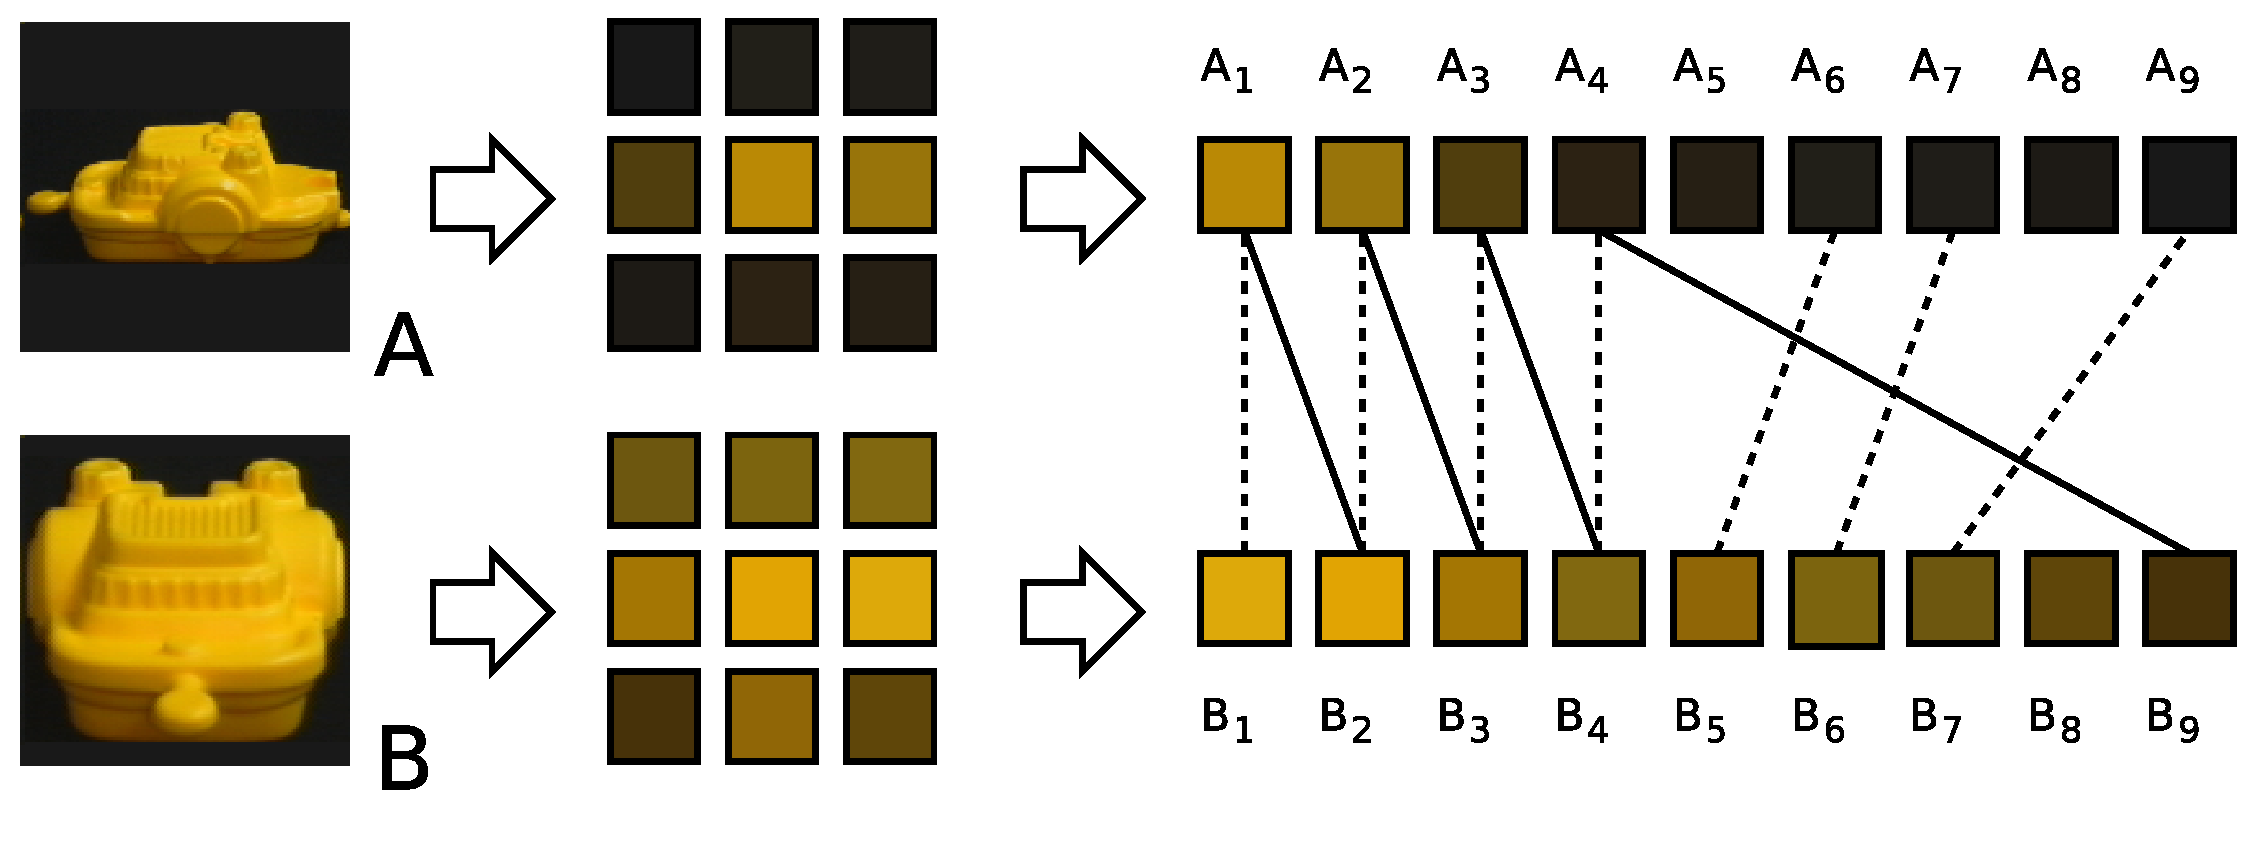
\includegraphics[width=10cm]{images/multires.eps}
\caption{\label{fig:multires}Constructie van een resolutie-onafhankelijke similariteitsmaat 
door gebruik van beeldonderdelen.}
\end{figure}

\begin{figure}[!bp]
\vspace{10pt}
\centering
\subfigure[]{
\includegraphics[width=0.3\textwidth]{images/multires_sim-matrix_1.eps}
\label{fig:multires_sim-matrix_1}
}
\subfigure[]{
\includegraphics[width=0.3\textwidth]{images/multires_sim-matrix_2.eps}
\label{fig:multires_sim-matrix_2}
}
\subfigure[]{
\includegraphics[width=0.3\textwidth]{images/multires_sim-matrix_beide.eps}
\label{fig:multires_sim-matrix_beide}
}
\caption{\label{fig:multires_sim-matrices}Het pad in de similariteitsmatrix van de beelden uit 
figuur~\ref{fig:multires} voor (a) $M(A,B)$, (b) $M(B,A)$ en (c) beide.}
\end{figure}

%\begin{table}
%\begin{center}
%\begin{tabular}{|c|ccccccccc|}
%\hline
%$\scriptstyle M_3(A_i,B_j)$	& $B_1$ & $B_2$ & $B_3$ & $B_4$ & $B_5$ & $B_6$ & $B_7$ & $B_8$ & $B_9$  \\
%\hline
%$A_1$ 	& $\mathbf{\scriptstyle 0.5198}$ & $\scriptstyle 0.4496$ & & & & & & & \\
%$A_2$ 	& & $\mathbf{\scriptstyle 0.4691}$ & $\scriptstyle 0.3859$ & & & & & & \\
%$A_3$ 	& & & $\scriptstyle 0.4133$ & $\mathbf{\scriptstyle 0.4404}$ & $\scriptstyle 0.3298$ & & & & \\
%$A_4$ 	& & & & & $\scriptstyle 0.3277$ & $\mathbf{\scriptstyle 0.4330}$ & $\scriptstyle 0.3648$ & & \\
%$A_5$ 	& & & & & & & $\mathbf{\scriptstyle 0.3849}$ & $\scriptstyle 0.3134$ & \\
%$A_6$ 	& & & & & & & & $\mathbf{\scriptstyle 0.3438}$ & $\scriptstyle 0.3427$ \\
%$A_7$ 	& & & & & & & & & $\mathbf{\scriptstyle 0.5066}$ \\
%\hline
%\end{tabular}
%\caption{\label{tab:multires}De similariteiten die berekend worden in de constructie die ge\"illustreerd wordt door figuur~\ref{fig:multires}.}
%\end{center}
%\end{table}

We kunnen de similariteiten tussen de verschillende beeldonderdelen van twee beelden
samenbrengen in een \defin{similariteitsmatrix}. Een dergelijke matrix kan grafisch 
voorgesteld worden als een grijswaardebeeld, waarbij de waarde van een beeldpunt evenredig is met
de overeenkomstige similariteit. Figuur~\ref{fig:multires_sim-matrix_1} toont het pad in de 
similariteitsmatrix van de beelden $A$ en $B$ uit figuur~\ref{fig:multires}, dat afgelopen wordt
bij het bepalen van $M(A,B)$.
De similariteiten die effectief berekend worden, hebben in die figuur een volle rand. Diegene 
die toegevoegd worden aan $S$ hebben een dikkere rand. Die laatste similariteiten 
worden in figuur~\ref{fig:multires} weergegeven als volle verbindingen tussen de
geordende beeldonderdelen. In figuur~\ref{fig:multires_sim-matrix_2} wordt het
pad voor het bepalen van $M(B,A)$ getoond. De similariteiten die daarbij toegevoegd 
worden aan $S$, worden in figuur~\ref{fig:multires} weergegeven met stippellijnen.
Figuur~\ref{fig:multires_sim-matrix_beide} toont beide paden tegelijkertijd. In die 
figuur zien we duidelijk dat het gemiddelde van $M(A,B)$ en $M(B,A)$ moet gebruikt 
worden om een symmetrische maat te bekomen.


\section{Experimentele observaties}

%In figuur~\ref{fig:pixelgeb_gggrs_en_cputimes} 
Tot slot van dit hoofdstuk vergelijken we enkele pixelgebaseerde similariteitsmaten.
Hoewel de beelden in onze testcollectie allemaal dezelfde resolutie hebben, zullen de
resoluties van de beelden die we in de praktijk gaan vergelijken vrijwel altijd verschillend zijn.
We beperken ons daarom tot resolutie-onafhankelijke similariteitsmaten. Die maten construeren
we op basis van een pixelgebaseerde maat, zoals besproken in \ref{sectie:res-onafh}. 
Voor het toepassen van de vaagsimilariteitsmaten op
intermediaire beelden of op beeldonderdelen, beschouwen we de drie manieren uit \ref{sectie:kleurbeelden_similariteitsmaten}:
(1) eerst omzetten naar grijswaardebeelden, 
(2) toepassen op de afzonderlijke kleurcomponenten en 
(3) traliegebaseerd. We gebruiken het gemiddelde om de similariteiten te aggregeren
bij de componentsgewijze aanpak.

\subsection{Resultaten van experimenten}

Figuur~\ref{fig:scaling_gggrs_en_cputimes} toont de GGGRs en de rekentijden voor de 
similariteitsmaten op basis van herschaling. De beste GGGR-waarde bekomen we 
bij componentsgewijze toepassing van $M_7$. In figuur~\ref{fig:results_beste_scaling} worden de resultaten van die maat
weergegeven. Die resultaten zijn vrij goed, maar dat is slechts een vertekend beeld van de
werkelijkheid. De beelden in onze testcollectie hebben immers allemaal dezelfde resolutie,
waardoor er nooit herschaling nodig is. Als er wel herschaald moet worden, dan kunnen
eventuele vervormingen zorgen voor slechtere performantie. 

Als we de similariteiten berekenen op intermediaire beelden van 8 pixels die 
geconstrueerd worden met behulp van NeuQuant en Wu kwantisatie, dan bekomen we
de meetresultaten die in figuur~\ref{fig:dom_colors_gggrs_en_cputimes} worden weergegeven.
De maten op basis van NeuQuant geven duidelijk minder goede resultaten. Dat is wellicht te wijten
aan het feit dat NeuQuant minder geschikt is voor kwantistatie naar een zeer klein aantal 
kleuren. Door $M_5$ componentsgewijs toe te passen, bekomen we in dit geval de beste resultaten. 
Figuur~\ref{fig:results_beste_dom_colors} toont de resultaten van de componentgebaseerde aanpak
in combinatie met Wu kwantisatie en $M_5$.

Intermediaire beelden op basis van kleurmomenten leiden tot de meetresultaten uit 
figuur \ref{fig:moments_gggrs_en_cputimes}. Hoewel het eigenlijk een zeer eenvoudige
techniek is, blijkt hij toch verrassend goed te werken. Ook hier leidt de
componentsgewijze aanpak tot de laagste GGGR-waarden. De combinatie met $M_9$ presteert
deze keer het best. Figuur~\ref{fig:results_beste_moments_pixelgeb} toont de resultaten
die we met die similariteitsmaat bekomen.

In figuur~\ref{fig:multires_gggrs_en_cputimes} worden de GGGRs en de rekentijden van
de similariteitsmaten op basis van beeldonderdelen van $8 \cdot 8$ pixels getoond.
De componentgebaseerde aanpak samen met
$M_{I_{3c}}$ geeft daarbij de beste GGGR-waarde. Zoals blijkt uit
figuur~\ref{fig:results_beste_multires_pixelgeb}, zijn de resultaten van die
maat niet zo overtuigend.

Uit de grafieken blijkt dat we de beste resultaten bekomen bij de similariteitsmaten 
die intermediaire beelden componentsgewijs vergelijken. Voor die maten proberen we, naast 
het rekenkundig gemiddelde, ook nog het minimum en het product voor het aggregeren 
van de similariteiten van de verschillende componenten. Figuur~\ref{fig:dom_colors_wu_comps_gggrs_en_cputimes}
en figuur~\ref{fig:moments_comps_gggrs_en_cputimes} tonen de resultaten van
die experimenten. We merken dat het minimum in bepaalde
gevallen beter werkt. Bovendien zien we in 
figuur~\ref{fig:results_beste_dom_colors_wu_comps_pixelgeb} en
figuur~\ref{fig:results_beste_moments_comps_pixelgeb} dat de beelden
die na de relevante beelden gerangschikt worden, vaak beter lijken op het voorbeeld als
we het minimum gebruiken. Beschouw bijvoorbeeld de resultaten voor het ``grijs bootje'' 
voorbeeld in figuur~\ref{fig:results_beste_moments_comps_pixelgeb}.
De beelden van de grijze tas, die deel uitmaken van die resultaten, zijn intu\"itief meer correct
dan de beelden die op dezelfde plaats gerangschikt worden in 
figuur~\ref{fig:results_beste_moments_pixelgeb}. 
\afterpage{\begin{figure}[p]
\centering
\includegraphics[width=\textwidth]{plots/scaling_gggrs_en_cputimes_filled.eps}
\vspace{1pt}
\caption{\label{fig:scaling_gggrs_en_cputimes}De GGGR-waarde en de rekentijd in ms 
voor elk van de similariteitsmaten op basis van herschaalde beelden.}
\end{figure}

\begin{figure}[p]
\vspace{5pt}
\centering
\begin{tabular}{m{11cm} | m{3cm} |}
\textbf{Eerste tien resultaten:} & \textbf{GGR:} \\
\vspace{4pt}
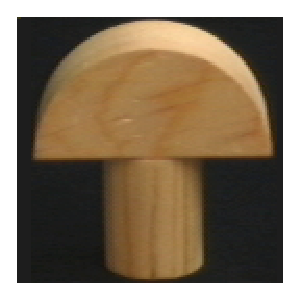
\includegraphics[width=1cm]{coil/beeld-0.eps}
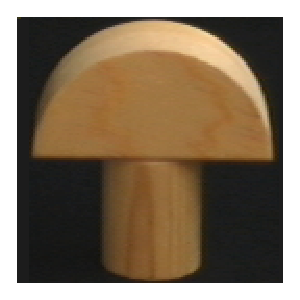
\includegraphics[width=1cm]{coil/beeld-1.eps}
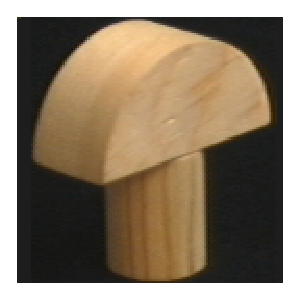
\includegraphics[width=1cm]{coil/beeld-3.eps}
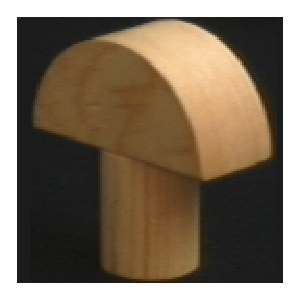
\includegraphics[width=1cm]{coil/beeld-4.eps}
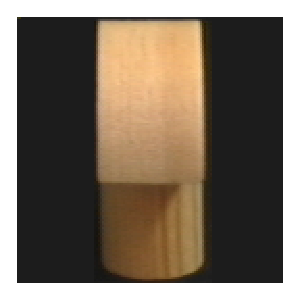
\includegraphics[width=1cm]{coil/beeld-2.eps}
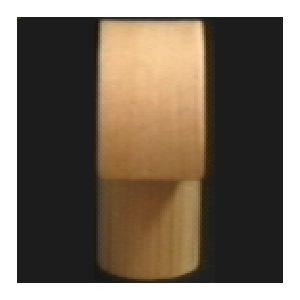
\includegraphics[width=1cm]{coil/beeld-5.eps}
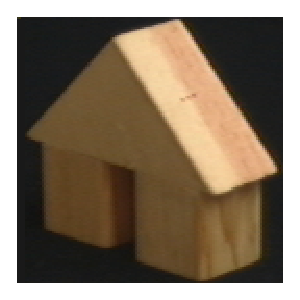
\includegraphics[width=1cm]{coil/beeld-46.eps}
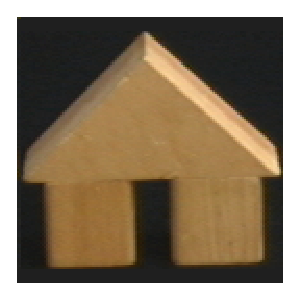
\includegraphics[width=1cm]{coil/beeld-42.eps}
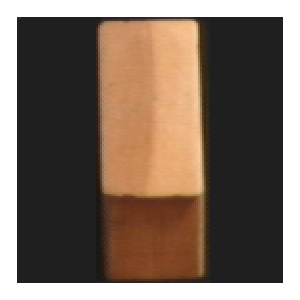
\includegraphics[width=1cm]{coil/beeld-44.eps}
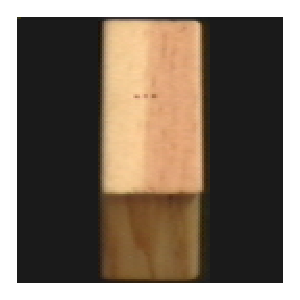
\includegraphics[width=1cm]{coil/beeld-47.eps}
& {\scriptsize 0.0}
\\
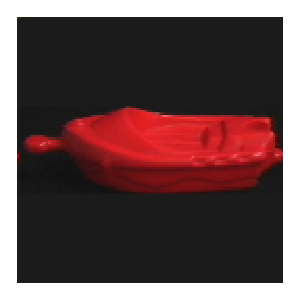
\includegraphics[width=1cm]{coil/beeld-18.eps}
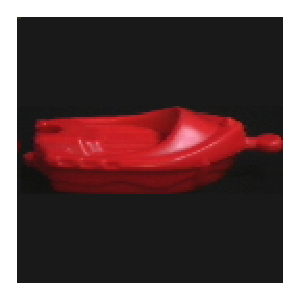
\includegraphics[width=1cm]{coil/beeld-19.eps}
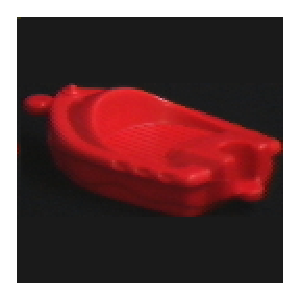
\includegraphics[width=1cm]{coil/beeld-22.eps}
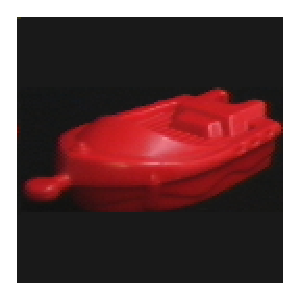
\includegraphics[width=1cm]{coil/beeld-21.eps}
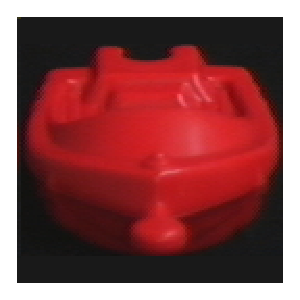
\includegraphics[width=1cm]{coil/beeld-20.eps}
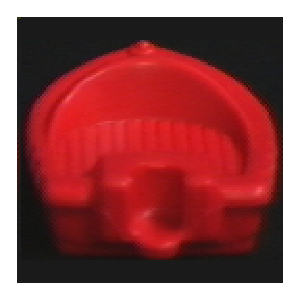
\includegraphics[width=1cm]{coil/beeld-23.eps}
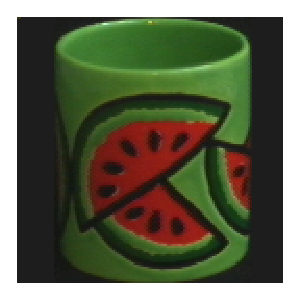
\includegraphics[width=1cm]{coil/beeld-32.eps}
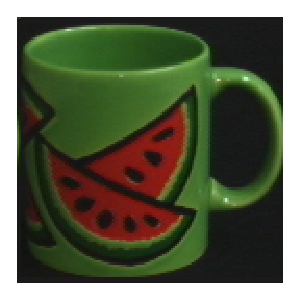
\includegraphics[width=1cm]{coil/beeld-30.eps}
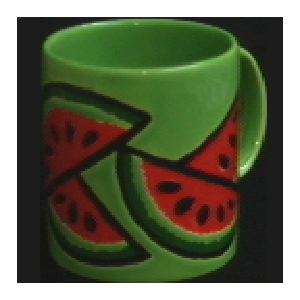
\includegraphics[width=1cm]{coil/beeld-33.eps}
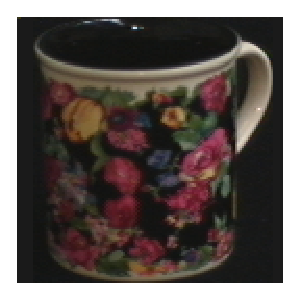
\includegraphics[width=1cm]{coil/beeld-63.eps}
& {\scriptsize 0.0}
\\
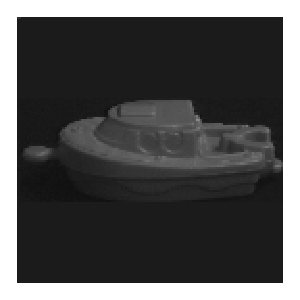
\includegraphics[width=1cm]{coil/beeld-24.eps}
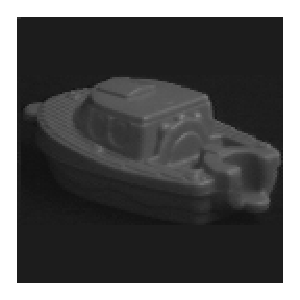
\includegraphics[width=1cm]{coil/beeld-25.eps}
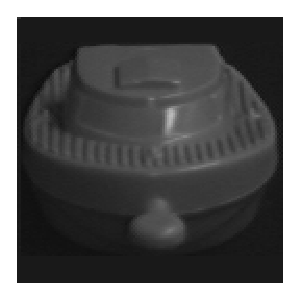
\includegraphics[width=1cm]{coil/beeld-28.eps}
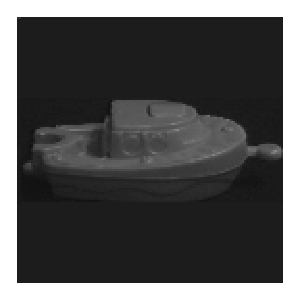
\includegraphics[width=1cm]{coil/beeld-27.eps}
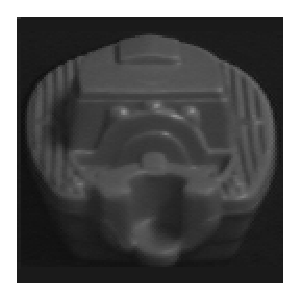
\includegraphics[width=1cm]{coil/beeld-26.eps}
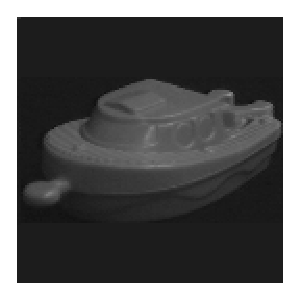
\includegraphics[width=1cm]{coil/beeld-29.eps}
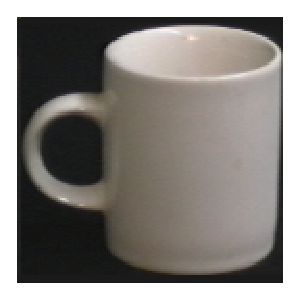
\includegraphics[width=1cm]{coil/beeld-37.eps}
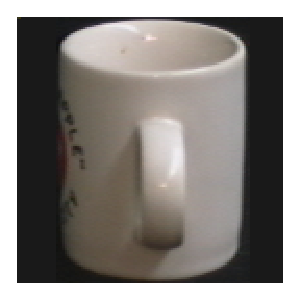
\includegraphics[width=1cm]{coil/beeld-41.eps}
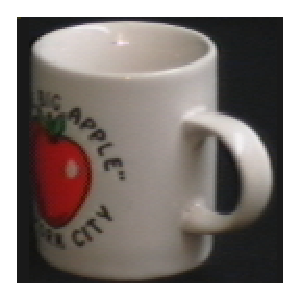
\includegraphics[width=1cm]{coil/beeld-40.eps}
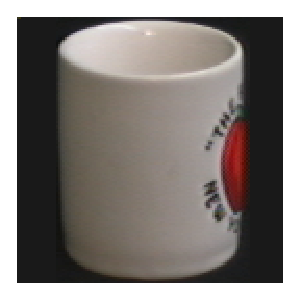
\includegraphics[width=1cm]{coil/beeld-38.eps}
& {\scriptsize 0.0}
\\
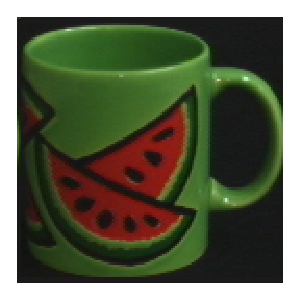
\includegraphics[width=1cm]{coil/beeld-30.eps}
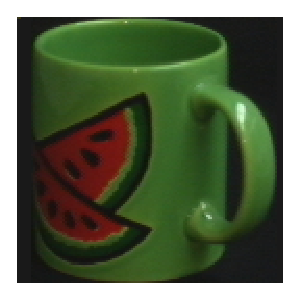
\includegraphics[width=1cm]{coil/beeld-34.eps}
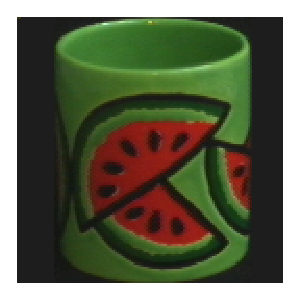
\includegraphics[width=1cm]{coil/beeld-32.eps}
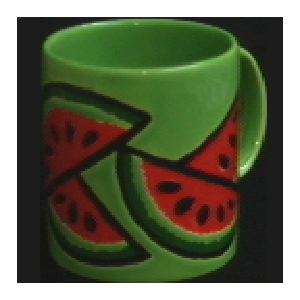
\includegraphics[width=1cm]{coil/beeld-33.eps}
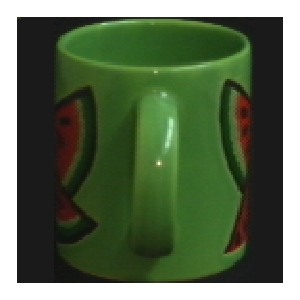
\includegraphics[width=1cm]{coil/beeld-35.eps}
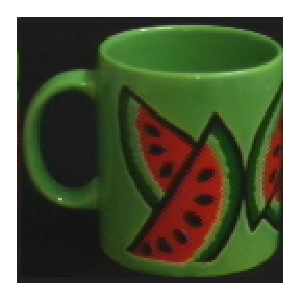
\includegraphics[width=1cm]{coil/beeld-31.eps}
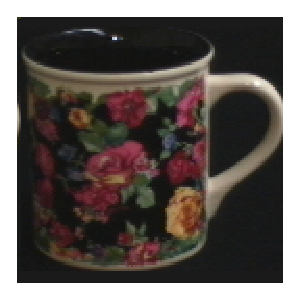
\includegraphics[width=1cm]{coil/beeld-60.eps}
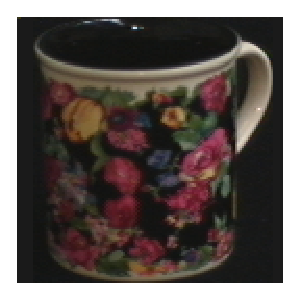
\includegraphics[width=1cm]{coil/beeld-63.eps}
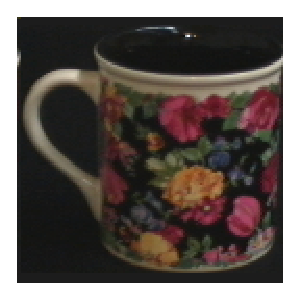
\includegraphics[width=1cm]{coil/beeld-61.eps}
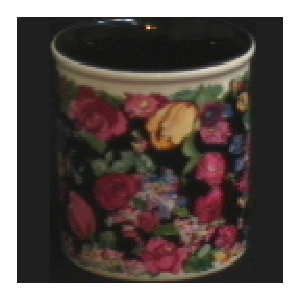
\includegraphics[width=1cm]{coil/beeld-62.eps}
& {\scriptsize 0.0}
\\
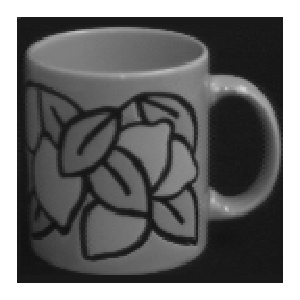
\includegraphics[width=1cm]{coil/beeld-48.eps}
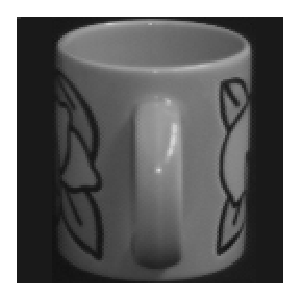
\includegraphics[width=1cm]{coil/beeld-50.eps}
\includegraphics[width=1cm]{coil/beeld-51.eps}
\includegraphics[width=1cm]{coil/beeld-52.eps}
\includegraphics[width=1cm]{coil/beeld-53.eps}
\includegraphics[width=1cm]{coil/beeld-49.eps}
\includegraphics[width=1cm]{coil/beeld-29.eps}
\includegraphics[width=1cm]{coil/beeld-26.eps}
\includegraphics[width=1cm]{coil/beeld-27.eps}
\includegraphics[width=1cm]{coil/beeld-28.eps}
& {\scriptsize 0.0}
\\
\includegraphics[width=1cm]{coil/beeld-54.eps}
\includegraphics[width=1cm]{coil/beeld-55.eps}
\includegraphics[width=1cm]{coil/beeld-57.eps}
\includegraphics[width=1cm]{coil/beeld-58.eps}
\includegraphics[width=1cm]{coil/beeld-56.eps}
\includegraphics[width=1cm]{coil/beeld-59.eps}
\includegraphics[width=1cm]{coil/beeld-35.eps}
\includegraphics[width=1cm]{coil/beeld-34.eps}
\includegraphics[width=1cm]{coil/beeld-30.eps}
\includegraphics[width=1cm]{coil/beeld-33.eps}
& {\scriptsize 0.0}
\\
\includegraphics[width=1cm]{coil/beeld-6.eps}
\includegraphics[width=1cm]{coil/beeld-9.eps}
\includegraphics[width=1cm]{coil/beeld-8.eps}
\includegraphics[width=1cm]{coil/beeld-10.eps}
\includegraphics[width=1cm]{coil/beeld-11.eps}
\includegraphics[width=1cm]{coil/beeld-2.eps}
\includegraphics[width=1cm]{coil/beeld-36.eps}
\includegraphics[width=1cm]{coil/beeld-5.eps}
\includegraphics[width=1cm]{coil/beeld-7.eps}
\includegraphics[width=1cm]{coil/beeld-47.eps}
& {\scriptsize 0.007142857142857143}
\\
\includegraphics[width=1cm]{coil/beeld-60.eps}
\includegraphics[width=1cm]{coil/beeld-63.eps}
\includegraphics[width=1cm]{coil/beeld-61.eps}
\includegraphics[width=1cm]{coil/beeld-62.eps}
\includegraphics[width=1cm]{coil/beeld-30.eps}
\includegraphics[width=1cm]{coil/beeld-64.eps}
\includegraphics[width=1cm]{coil/beeld-32.eps}
\includegraphics[width=1cm]{coil/beeld-65.eps}
\includegraphics[width=1cm]{coil/beeld-33.eps}
\includegraphics[width=1cm]{coil/beeld-31.eps}
& {\scriptsize 0.007142857142857143}
\\
\includegraphics[width=1cm]{coil/beeld-36.eps}
\includegraphics[width=1cm]{coil/beeld-40.eps}
\includegraphics[width=1cm]{coil/beeld-39.eps}
\includegraphics[width=1cm]{coil/beeld-38.eps}
\includegraphics[width=1cm]{coil/beeld-10.eps}
\includegraphics[width=1cm]{coil/beeld-41.eps}
\includegraphics[width=1cm]{coil/beeld-3.eps}
\includegraphics[width=1cm]{coil/beeld-11.eps}
\includegraphics[width=1cm]{coil/beeld-6.eps}
\includegraphics[width=1cm]{coil/beeld-24.eps}
& {\scriptsize 0.016666666666666666}
\\
\includegraphics[width=1cm]{coil/beeld-42.eps}
\includegraphics[width=1cm]{coil/beeld-43.eps}
\includegraphics[width=1cm]{coil/beeld-46.eps}
\includegraphics[width=1cm]{coil/beeld-0.eps}
\includegraphics[width=1cm]{coil/beeld-45.eps}
\includegraphics[width=1cm]{coil/beeld-3.eps}
\includegraphics[width=1cm]{coil/beeld-1.eps}
\includegraphics[width=1cm]{coil/beeld-4.eps}
\includegraphics[width=1cm]{coil/beeld-2.eps}
\includegraphics[width=1cm]{coil/beeld-10.eps}
& {\scriptsize 0.0380952380952381}
\\
\includegraphics[width=1cm]{coil/beeld-12.eps}
\includegraphics[width=1cm]{coil/beeld-13.eps}
\includegraphics[width=1cm]{coil/beeld-16.eps}
\includegraphics[width=1cm]{coil/beeld-15.eps}
\includegraphics[width=1cm]{coil/beeld-21.eps}
\includegraphics[width=1cm]{coil/beeld-22.eps}
\includegraphics[width=1cm]{coil/beeld-18.eps}
\includegraphics[width=1cm]{coil/beeld-19.eps}
\includegraphics[width=1cm]{coil/beeld-30.eps}
\includegraphics[width=1cm]{coil/beeld-33.eps}
& {\scriptsize 0.15}
\\
\end{tabular}
\vspace{5pt}
\caption{\label{fig:results_beste_scaling}De GGR-waarde en de eerste tien resultaten voor elk 
voorbeeld bij de similariteitsmaat die we bekomen door herschaalde beelden componentsgewijs 
te vergelijken met behulp van $M_7$ en het gemiddelde.}
\end{figure}

\begin{figure}[p]
\vspace{5pt}
\centering
\subfigure[]{
\begin{minipage}{\textwidth}
\includegraphics[width=\textwidth]{plots/dom_colors_neuquant_gggrs_en_cputimes_filled.eps}
\vspace{2pt}
\end{minipage}
\label{fig:dom_colors_neuquant_gggrs_en_cputimes}
}
\subfigure[]{
\begin{minipage}{\textwidth}
\includegraphics[width=\textwidth]{plots/dom_colors_wu_gggrs_en_cputimes_filled.eps}
\vspace{2pt}
\end{minipage}
\label{fig:dom_colors_wu_gggrs_en_cputimes}
}
\caption{\label{fig:dom_colors_gggrs_en_cputimes}De GGGR-waarde en de rekentijd in ms 
voor elk van de similariteitsmaten die gebruik maken 
van op basis van (a) NeuQuant en (b) Wu kwantisatie geconstrueerde intermediaire beelden.}
\end{figure}

\begin{figure}[p]
\vspace{5pt}
\centering
\begin{tabular}{m{11cm} | m{3cm} |}
\textbf{Eerste tien resultaten:} & \textbf{GGR:} \\
\vspace{4pt}
\includegraphics[width=1cm]{coil/beeld-12.eps}
\includegraphics[width=1cm]{coil/beeld-17.eps}
\includegraphics[width=1cm]{coil/beeld-13.eps}
\includegraphics[width=1cm]{coil/beeld-15.eps}
\includegraphics[width=1cm]{coil/beeld-14.eps}
\includegraphics[width=1cm]{coil/beeld-16.eps}
\includegraphics[width=1cm]{coil/beeld-42.eps}
\includegraphics[width=1cm]{coil/beeld-5.eps}
\includegraphics[width=1cm]{coil/beeld-4.eps}
\includegraphics[width=1cm]{coil/beeld-1.eps}
& {\scriptsize 0.0}
\\
\includegraphics[width=1cm]{coil/beeld-18.eps}
\includegraphics[width=1cm]{coil/beeld-20.eps}
\includegraphics[width=1cm]{coil/beeld-23.eps}
\includegraphics[width=1cm]{coil/beeld-22.eps}
\includegraphics[width=1cm]{coil/beeld-21.eps}
\includegraphics[width=1cm]{coil/beeld-19.eps}
\includegraphics[width=1cm]{coil/beeld-45.eps}
\includegraphics[width=1cm]{coil/beeld-31.eps}
\includegraphics[width=1cm]{coil/beeld-30.eps}
\includegraphics[width=1cm]{coil/beeld-33.eps}
& {\scriptsize 0.0}
\\
\includegraphics[width=1cm]{coil/beeld-30.eps}
\includegraphics[width=1cm]{coil/beeld-31.eps}
\includegraphics[width=1cm]{coil/beeld-33.eps}
\includegraphics[width=1cm]{coil/beeld-32.eps}
\includegraphics[width=1cm]{coil/beeld-35.eps}
\includegraphics[width=1cm]{coil/beeld-34.eps}
\includegraphics[width=1cm]{coil/beeld-61.eps}
\includegraphics[width=1cm]{coil/beeld-60.eps}
\includegraphics[width=1cm]{coil/beeld-63.eps}
\includegraphics[width=1cm]{coil/beeld-62.eps}
& {\scriptsize 0.0}
\\
\includegraphics[width=1cm]{coil/beeld-54.eps}
\includegraphics[width=1cm]{coil/beeld-58.eps}
\includegraphics[width=1cm]{coil/beeld-59.eps}
\includegraphics[width=1cm]{coil/beeld-56.eps}
\includegraphics[width=1cm]{coil/beeld-55.eps}
\includegraphics[width=1cm]{coil/beeld-57.eps}
\includegraphics[width=1cm]{coil/beeld-35.eps}
\includegraphics[width=1cm]{coil/beeld-34.eps}
\includegraphics[width=1cm]{coil/beeld-32.eps}
\includegraphics[width=1cm]{coil/beeld-33.eps}
& {\scriptsize 0.0}
\\
\includegraphics[width=1cm]{coil/beeld-24.eps}
\includegraphics[width=1cm]{coil/beeld-28.eps}
\includegraphics[width=1cm]{coil/beeld-29.eps}
\includegraphics[width=1cm]{coil/beeld-25.eps}
\includegraphics[width=1cm]{coil/beeld-27.eps}
\includegraphics[width=1cm]{coil/beeld-37.eps}
\includegraphics[width=1cm]{coil/beeld-41.eps}
\includegraphics[width=1cm]{coil/beeld-26.eps}
\includegraphics[width=1cm]{coil/beeld-48.eps}
\includegraphics[width=1cm]{coil/beeld-51.eps}
& {\scriptsize 0.004761904761904762}
\\
\includegraphics[width=1cm]{coil/beeld-48.eps}
\includegraphics[width=1cm]{coil/beeld-51.eps}
\includegraphics[width=1cm]{coil/beeld-50.eps}
\includegraphics[width=1cm]{coil/beeld-52.eps}
\includegraphics[width=1cm]{coil/beeld-26.eps}
\includegraphics[width=1cm]{coil/beeld-49.eps}
\includegraphics[width=1cm]{coil/beeld-27.eps}
\includegraphics[width=1cm]{coil/beeld-53.eps}
\includegraphics[width=1cm]{coil/beeld-37.eps}
\includegraphics[width=1cm]{coil/beeld-25.eps}
& {\scriptsize 0.007142857142857143}
\\
\includegraphics[width=1cm]{coil/beeld-60.eps}
\includegraphics[width=1cm]{coil/beeld-63.eps}
\includegraphics[width=1cm]{coil/beeld-62.eps}
\includegraphics[width=1cm]{coil/beeld-61.eps}
\includegraphics[width=1cm]{coil/beeld-7.eps}
\includegraphics[width=1cm]{coil/beeld-64.eps}
\includegraphics[width=1cm]{coil/beeld-8.eps}
\includegraphics[width=1cm]{coil/beeld-9.eps}
\includegraphics[width=1cm]{coil/beeld-65.eps}
\includegraphics[width=1cm]{coil/beeld-0.eps}
& {\scriptsize 0.009523809523809525}
\\
\includegraphics[width=1cm]{coil/beeld-6.eps}
\includegraphics[width=1cm]{coil/beeld-10.eps}
\includegraphics[width=1cm]{coil/beeld-40.eps}
\includegraphics[width=1cm]{coil/beeld-65.eps}
\includegraphics[width=1cm]{coil/beeld-11.eps}
\includegraphics[width=1cm]{coil/beeld-38.eps}
\includegraphics[width=1cm]{coil/beeld-9.eps}
\includegraphics[width=1cm]{coil/beeld-39.eps}
\includegraphics[width=1cm]{coil/beeld-8.eps}
\includegraphics[width=1cm]{coil/beeld-64.eps}
& {\scriptsize 0.0380952380952381}
\\
\includegraphics[width=1cm]{coil/beeld-0.eps}
\includegraphics[width=1cm]{coil/beeld-2.eps}
\includegraphics[width=1cm]{coil/beeld-46.eps}
\includegraphics[width=1cm]{coil/beeld-44.eps}
\includegraphics[width=1cm]{coil/beeld-45.eps}
\includegraphics[width=1cm]{coil/beeld-1.eps}
\includegraphics[width=1cm]{coil/beeld-43.eps}
\includegraphics[width=1cm]{coil/beeld-47.eps}
\includegraphics[width=1cm]{coil/beeld-3.eps}
\includegraphics[width=1cm]{coil/beeld-4.eps}
& {\scriptsize 0.04523809523809524}
\\
\includegraphics[width=1cm]{coil/beeld-36.eps}
\includegraphics[width=1cm]{coil/beeld-11.eps}
\includegraphics[width=1cm]{coil/beeld-40.eps}
\includegraphics[width=1cm]{coil/beeld-39.eps}
\includegraphics[width=1cm]{coil/beeld-38.eps}
\includegraphics[width=1cm]{coil/beeld-10.eps}
\includegraphics[width=1cm]{coil/beeld-6.eps}
\includegraphics[width=1cm]{coil/beeld-46.eps}
\includegraphics[width=1cm]{coil/beeld-41.eps}
\includegraphics[width=1cm]{coil/beeld-47.eps}
& {\scriptsize 0.047619047619047616}
\\
\includegraphics[width=1cm]{coil/beeld-42.eps}
\includegraphics[width=1cm]{coil/beeld-5.eps}
\includegraphics[width=1cm]{coil/beeld-4.eps}
\includegraphics[width=1cm]{coil/beeld-3.eps}
\includegraphics[width=1cm]{coil/beeld-43.eps}
\includegraphics[width=1cm]{coil/beeld-47.eps}
\includegraphics[width=1cm]{coil/beeld-1.eps}
\includegraphics[width=1cm]{coil/beeld-46.eps}
\includegraphics[width=1cm]{coil/beeld-44.eps}
\includegraphics[width=1cm]{coil/beeld-2.eps}
& {\scriptsize 0.047619047619047616}
\\
\end{tabular}
\vspace{5pt}
\caption{\label{fig:results_beste_dom_colors}De GGR-waarde en de eerste tien resultaten voor elk 
voorbeeld bij de similariteitsmaat die we bekomen door op basis van Wu 
kwantisatie geconstrueerde intermediaire beelden componentsgewijs te vergelijken met behulp van 
$M_5$ en het gemiddelde.}
\end{figure}

\clearpage

\begin{figure}[p]
% \caption{\label{fig:moments_gggrs_en_cputimes}De GGGR-waarde en de gebruikte rekentijd in ms 
% voor elk van de resolutie-onafhankelijke pixelgebaseerde similariteitsmaten die gebruik maken 
% van op basis van kleurmomenten geconstrueerde intermediaire beelden.}
\centering
\includegraphics[width=\textwidth]{plots/moments_gggrs_en_cputimes_filled.eps}
\vspace{1pt}
\caption{\label{fig:moments_gggrs_en_cputimes}De GGGR-waarde en de rekentijd in ms
voor elk van de similariteitsmaten die gebruik maken
van op basis van kleurmomenten geconstrueerde intermediaire beelden.}
\end{figure}

\begin{figure}[p]
\vspace{5pt}
\centering
\begin{tabular}{m{11cm} | m{3cm} |}
\textbf{Eerste tien resultaten:} & \textbf{GGR:} \\
\vspace{4pt}
\includegraphics[width=1cm]{coil/beeld-12.eps}
\includegraphics[width=1cm]{coil/beeld-13.eps}
\includegraphics[width=1cm]{coil/beeld-16.eps}
\includegraphics[width=1cm]{coil/beeld-15.eps}
\includegraphics[width=1cm]{coil/beeld-17.eps}
\includegraphics[width=1cm]{coil/beeld-14.eps}
\includegraphics[width=1cm]{coil/beeld-44.eps}
\includegraphics[width=1cm]{coil/beeld-1.eps}
\includegraphics[width=1cm]{coil/beeld-5.eps}
\includegraphics[width=1cm]{coil/beeld-4.eps}
& {\scriptsize 0.0}
\\
\includegraphics[width=1cm]{coil/beeld-6.eps}
\includegraphics[width=1cm]{coil/beeld-9.eps}
\includegraphics[width=1cm]{coil/beeld-8.eps}
\includegraphics[width=1cm]{coil/beeld-10.eps}
\includegraphics[width=1cm]{coil/beeld-7.eps}
\includegraphics[width=1cm]{coil/beeld-11.eps}
\includegraphics[width=1cm]{coil/beeld-65.eps}
\includegraphics[width=1cm]{coil/beeld-64.eps}
\includegraphics[width=1cm]{coil/beeld-4.eps}
\includegraphics[width=1cm]{coil/beeld-43.eps}
& {\scriptsize 0.0}
\\
\includegraphics[width=1cm]{coil/beeld-18.eps}
\includegraphics[width=1cm]{coil/beeld-22.eps}
\includegraphics[width=1cm]{coil/beeld-23.eps}
\includegraphics[width=1cm]{coil/beeld-21.eps}
\includegraphics[width=1cm]{coil/beeld-20.eps}
\includegraphics[width=1cm]{coil/beeld-19.eps}
\includegraphics[width=1cm]{coil/beeld-12.eps}
\includegraphics[width=1cm]{coil/beeld-13.eps}
\includegraphics[width=1cm]{coil/beeld-16.eps}
\includegraphics[width=1cm]{coil/beeld-15.eps}
& {\scriptsize 0.0}
\\
\includegraphics[width=1cm]{coil/beeld-24.eps}
\includegraphics[width=1cm]{coil/beeld-25.eps}
\includegraphics[width=1cm]{coil/beeld-28.eps}
\includegraphics[width=1cm]{coil/beeld-27.eps}
\includegraphics[width=1cm]{coil/beeld-26.eps}
\includegraphics[width=1cm]{coil/beeld-29.eps}
\includegraphics[width=1cm]{coil/beeld-8.eps}
\includegraphics[width=1cm]{coil/beeld-7.eps}
\includegraphics[width=1cm]{coil/beeld-9.eps}
\includegraphics[width=1cm]{coil/beeld-6.eps}
& {\scriptsize 0.0}
\\
\includegraphics[width=1cm]{coil/beeld-30.eps}
\includegraphics[width=1cm]{coil/beeld-31.eps}
\includegraphics[width=1cm]{coil/beeld-32.eps}
\includegraphics[width=1cm]{coil/beeld-33.eps}
\includegraphics[width=1cm]{coil/beeld-34.eps}
\includegraphics[width=1cm]{coil/beeld-35.eps}
\includegraphics[width=1cm]{coil/beeld-61.eps}
\includegraphics[width=1cm]{coil/beeld-63.eps}
\includegraphics[width=1cm]{coil/beeld-62.eps}
\includegraphics[width=1cm]{coil/beeld-60.eps}
& {\scriptsize 0.0}
\\
\includegraphics[width=1cm]{coil/beeld-36.eps}
\includegraphics[width=1cm]{coil/beeld-39.eps}
\includegraphics[width=1cm]{coil/beeld-40.eps}
\includegraphics[width=1cm]{coil/beeld-41.eps}
\includegraphics[width=1cm]{coil/beeld-37.eps}
\includegraphics[width=1cm]{coil/beeld-38.eps}
\includegraphics[width=1cm]{coil/beeld-11.eps}
\includegraphics[width=1cm]{coil/beeld-10.eps}
\includegraphics[width=1cm]{coil/beeld-3.eps}
\includegraphics[width=1cm]{coil/beeld-46.eps}
& {\scriptsize 0.0}
\\
\includegraphics[width=1cm]{coil/beeld-48.eps}
\includegraphics[width=1cm]{coil/beeld-49.eps}
\includegraphics[width=1cm]{coil/beeld-50.eps}
\includegraphics[width=1cm]{coil/beeld-51.eps}
\includegraphics[width=1cm]{coil/beeld-53.eps}
\includegraphics[width=1cm]{coil/beeld-52.eps}
\includegraphics[width=1cm]{coil/beeld-37.eps}
\includegraphics[width=1cm]{coil/beeld-40.eps}
\includegraphics[width=1cm]{coil/beeld-41.eps}
\includegraphics[width=1cm]{coil/beeld-38.eps}
& {\scriptsize 0.0}
\\
\includegraphics[width=1cm]{coil/beeld-54.eps}
\includegraphics[width=1cm]{coil/beeld-55.eps}
\includegraphics[width=1cm]{coil/beeld-57.eps}
\includegraphics[width=1cm]{coil/beeld-58.eps}
\includegraphics[width=1cm]{coil/beeld-56.eps}
\includegraphics[width=1cm]{coil/beeld-59.eps}
\includegraphics[width=1cm]{coil/beeld-35.eps}
\includegraphics[width=1cm]{coil/beeld-32.eps}
\includegraphics[width=1cm]{coil/beeld-31.eps}
\includegraphics[width=1cm]{coil/beeld-33.eps}
& {\scriptsize 0.0}
\\
\includegraphics[width=1cm]{coil/beeld-60.eps}
\includegraphics[width=1cm]{coil/beeld-63.eps}
\includegraphics[width=1cm]{coil/beeld-61.eps}
\includegraphics[width=1cm]{coil/beeld-62.eps}
\includegraphics[width=1cm]{coil/beeld-64.eps}
\includegraphics[width=1cm]{coil/beeld-65.eps}
\includegraphics[width=1cm]{coil/beeld-43.eps}
\includegraphics[width=1cm]{coil/beeld-7.eps}
\includegraphics[width=1cm]{coil/beeld-1.eps}
\includegraphics[width=1cm]{coil/beeld-32.eps}
& {\scriptsize 0.0}
\\
\includegraphics[width=1cm]{coil/beeld-0.eps}
\includegraphics[width=1cm]{coil/beeld-42.eps}
\includegraphics[width=1cm]{coil/beeld-1.eps}
\includegraphics[width=1cm]{coil/beeld-4.eps}
\includegraphics[width=1cm]{coil/beeld-44.eps}
\includegraphics[width=1cm]{coil/beeld-43.eps}
\includegraphics[width=1cm]{coil/beeld-2.eps}
\includegraphics[width=1cm]{coil/beeld-5.eps}
\includegraphics[width=1cm]{coil/beeld-46.eps}
\includegraphics[width=1cm]{coil/beeld-3.eps}
& {\scriptsize 0.02857142857142857}
\\
\includegraphics[width=1cm]{coil/beeld-42.eps}
\includegraphics[width=1cm]{coil/beeld-0.eps}
\includegraphics[width=1cm]{coil/beeld-1.eps}
\includegraphics[width=1cm]{coil/beeld-43.eps}
\includegraphics[width=1cm]{coil/beeld-4.eps}
\includegraphics[width=1cm]{coil/beeld-44.eps}
\includegraphics[width=1cm]{coil/beeld-2.eps}
\includegraphics[width=1cm]{coil/beeld-5.eps}
\includegraphics[width=1cm]{coil/beeld-3.eps}
\includegraphics[width=1cm]{coil/beeld-45.eps}
& {\scriptsize 0.06428571428571428}
\\
\end{tabular}
\vspace{5pt}
\caption{\label{fig:results_beste_moments_pixelgeb}De GGR-waarde en de eerste tien resultaten 
voor elk voorbeeld bij de similariteitsmaat die we bekomen door op 
basis van kleurmomenten geconstrueerde intermediaire beelden componentsgewijs te vergelijken 
met behulp van $M_{9}$ en het gemiddelde.}
\end{figure}

%\clearpage

\begin{figure}[p]
\centering
\includegraphics[width=\textwidth]{plots/multires_gggrs_en_cputimes_filled.eps}
\vspace{1pt}
\caption{\label{fig:multires_gggrs_en_cputimes}De GGGR-waarde en de rekentijd in ms 
voor elk van de similariteitsmaten op basis van 
beeldonderdelen.}
\end{figure}

\begin{figure}[p]
\vspace{5pt}
\centering
\begin{tabular}{m{11cm} | m{3cm} |}
\textbf{Eerste tien resultaten:} & \textbf{GGR:} \\
\vspace{4pt}
\includegraphics[width=1cm]{coil/beeld-18.eps}
\includegraphics[width=1cm]{coil/beeld-22.eps}
\includegraphics[width=1cm]{coil/beeld-21.eps}
\includegraphics[width=1cm]{coil/beeld-19.eps}
\includegraphics[width=1cm]{coil/beeld-20.eps}
\includegraphics[width=1cm]{coil/beeld-23.eps}
\includegraphics[width=1cm]{coil/beeld-61.eps}
\includegraphics[width=1cm]{coil/beeld-63.eps}
\includegraphics[width=1cm]{coil/beeld-62.eps}
\includegraphics[width=1cm]{coil/beeld-60.eps}
& {\scriptsize 0.0}
\\
\includegraphics[width=1cm]{coil/beeld-24.eps}
\includegraphics[width=1cm]{coil/beeld-25.eps}
\includegraphics[width=1cm]{coil/beeld-28.eps}
\includegraphics[width=1cm]{coil/beeld-27.eps}
\includegraphics[width=1cm]{coil/beeld-26.eps}
\includegraphics[width=1cm]{coil/beeld-29.eps}
\includegraphics[width=1cm]{coil/beeld-10.eps}
\includegraphics[width=1cm]{coil/beeld-38.eps}
\includegraphics[width=1cm]{coil/beeld-11.eps}
\includegraphics[width=1cm]{coil/beeld-9.eps}
& {\scriptsize 0.0}
\\
\includegraphics[width=1cm]{coil/beeld-30.eps}
\includegraphics[width=1cm]{coil/beeld-34.eps}
\includegraphics[width=1cm]{coil/beeld-35.eps}
\includegraphics[width=1cm]{coil/beeld-31.eps}
\includegraphics[width=1cm]{coil/beeld-33.eps}
\includegraphics[width=1cm]{coil/beeld-32.eps}
\includegraphics[width=1cm]{coil/beeld-55.eps}
\includegraphics[width=1cm]{coil/beeld-61.eps}
\includegraphics[width=1cm]{coil/beeld-54.eps}
\includegraphics[width=1cm]{coil/beeld-60.eps}
& {\scriptsize 0.0}
\\
\includegraphics[width=1cm]{coil/beeld-36.eps}
\includegraphics[width=1cm]{coil/beeld-38.eps}
\includegraphics[width=1cm]{coil/beeld-41.eps}
\includegraphics[width=1cm]{coil/beeld-37.eps}
\includegraphics[width=1cm]{coil/beeld-27.eps}
\includegraphics[width=1cm]{coil/beeld-39.eps}
\includegraphics[width=1cm]{coil/beeld-4.eps}
\includegraphics[width=1cm]{coil/beeld-40.eps}
\includegraphics[width=1cm]{coil/beeld-24.eps}
\includegraphics[width=1cm]{coil/beeld-11.eps}
& {\scriptsize 0.007142857142857143}
\\
\includegraphics[width=1cm]{coil/beeld-48.eps}
\includegraphics[width=1cm]{coil/beeld-27.eps}
\includegraphics[width=1cm]{coil/beeld-53.eps}
\includegraphics[width=1cm]{coil/beeld-50.eps}
\includegraphics[width=1cm]{coil/beeld-52.eps}
\includegraphics[width=1cm]{coil/beeld-51.eps}
\includegraphics[width=1cm]{coil/beeld-49.eps}
\includegraphics[width=1cm]{coil/beeld-26.eps}
\includegraphics[width=1cm]{coil/beeld-28.eps}
\includegraphics[width=1cm]{coil/beeld-29.eps}
& {\scriptsize 0.011904761904761904}
\\
\includegraphics[width=1cm]{coil/beeld-12.eps}
\includegraphics[width=1cm]{coil/beeld-13.eps}
\includegraphics[width=1cm]{coil/beeld-15.eps}
\includegraphics[width=1cm]{coil/beeld-16.eps}
\includegraphics[width=1cm]{coil/beeld-30.eps}
\includegraphics[width=1cm]{coil/beeld-20.eps}
\includegraphics[width=1cm]{coil/beeld-34.eps}
\includegraphics[width=1cm]{coil/beeld-31.eps}
\includegraphics[width=1cm]{coil/beeld-17.eps}
\includegraphics[width=1cm]{coil/beeld-14.eps}
& {\scriptsize 0.01904761904761905}
\\
\includegraphics[width=1cm]{coil/beeld-54.eps}
\includegraphics[width=1cm]{coil/beeld-55.eps}
\includegraphics[width=1cm]{coil/beeld-57.eps}
\includegraphics[width=1cm]{coil/beeld-58.eps}
\includegraphics[width=1cm]{coil/beeld-34.eps}
\includegraphics[width=1cm]{coil/beeld-31.eps}
\includegraphics[width=1cm]{coil/beeld-30.eps}
\includegraphics[width=1cm]{coil/beeld-35.eps}
\includegraphics[width=1cm]{coil/beeld-59.eps}
\includegraphics[width=1cm]{coil/beeld-56.eps}
& {\scriptsize 0.01904761904761905}
\\
\includegraphics[width=1cm]{coil/beeld-60.eps}
\includegraphics[width=1cm]{coil/beeld-61.eps}
\includegraphics[width=1cm]{coil/beeld-63.eps}
\includegraphics[width=1cm]{coil/beeld-62.eps}
\includegraphics[width=1cm]{coil/beeld-30.eps}
\includegraphics[width=1cm]{coil/beeld-34.eps}
\includegraphics[width=1cm]{coil/beeld-31.eps}
\includegraphics[width=1cm]{coil/beeld-64.eps}
\includegraphics[width=1cm]{coil/beeld-35.eps}
\includegraphics[width=1cm]{coil/beeld-33.eps}
& {\scriptsize 0.02142857142857143}
\\
\includegraphics[width=1cm]{coil/beeld-0.eps}
\includegraphics[width=1cm]{coil/beeld-1.eps}
\includegraphics[width=1cm]{coil/beeld-42.eps}
\includegraphics[width=1cm]{coil/beeld-5.eps}
\includegraphics[width=1cm]{coil/beeld-43.eps}
\includegraphics[width=1cm]{coil/beeld-2.eps}
\includegraphics[width=1cm]{coil/beeld-44.eps}
\includegraphics[width=1cm]{coil/beeld-4.eps}
\includegraphics[width=1cm]{coil/beeld-64.eps}
\includegraphics[width=1cm]{coil/beeld-3.eps}
& {\scriptsize 0.023809523809523808}
\\
\includegraphics[width=1cm]{coil/beeld-6.eps}
\includegraphics[width=1cm]{coil/beeld-64.eps}
\includegraphics[width=1cm]{coil/beeld-7.eps}
\includegraphics[width=1cm]{coil/beeld-8.eps}
\includegraphics[width=1cm]{coil/beeld-65.eps}
\includegraphics[width=1cm]{coil/beeld-9.eps}
\includegraphics[width=1cm]{coil/beeld-25.eps}
\includegraphics[width=1cm]{coil/beeld-24.eps}
\includegraphics[width=1cm]{coil/beeld-60.eps}
\includegraphics[width=1cm]{coil/beeld-61.eps}
& {\scriptsize 0.06190476190476191}
\\
\includegraphics[width=1cm]{coil/beeld-42.eps}
\includegraphics[width=1cm]{coil/beeld-0.eps}
\includegraphics[width=1cm]{coil/beeld-1.eps}
\includegraphics[width=1cm]{coil/beeld-5.eps}
\includegraphics[width=1cm]{coil/beeld-43.eps}
\includegraphics[width=1cm]{coil/beeld-3.eps}
\includegraphics[width=1cm]{coil/beeld-2.eps}
\includegraphics[width=1cm]{coil/beeld-44.eps}
\includegraphics[width=1cm]{coil/beeld-4.eps}
\includegraphics[width=1cm]{coil/beeld-64.eps}
& {\scriptsize 0.1}
\\
\end{tabular}
\vspace{5pt}
\caption{\label{fig:results_beste_multires_pixelgeb}De GGR-waarde en de eerste tien resultaten 
voor elk voorbeeld bij de similariteitsmaat die we bekomen door 
beeldonderdelen componentsgewijs te vergelijken met behulp van $M_{I_{3c}}$ en het gemiddelde.}
\end{figure}

\begin{figure}[p]
\centering
\includegraphics[width=\textwidth]{plots/dom_colors_wu_comps_gggrs_en_cputimes_filled.eps}
\vspace{1pt}
\caption{\label{fig:dom_colors_wu_comps_gggrs_en_cputimes}De GGGR-waarde en de rekentijd in ms 
voor enkele similariteitsmaten die
op basis van Wu kwantisatie geconstrueerde intermediaire beelden componentsgewijs vergelijken.}
\end{figure}

\begin{figure}[p]
\vspace{5pt}
\centering
\begin{tabular}{m{11cm} | m{3cm} |}
\textbf{Eerste tien resultaten:} & \textbf{GGR:} \\
\vspace{4pt}
\includegraphics[width=1cm]{coil/beeld-12.eps}
\includegraphics[width=1cm]{coil/beeld-13.eps}
\includegraphics[width=1cm]{coil/beeld-15.eps}
\includegraphics[width=1cm]{coil/beeld-17.eps}
\includegraphics[width=1cm]{coil/beeld-14.eps}
\includegraphics[width=1cm]{coil/beeld-16.eps}
\includegraphics[width=1cm]{coil/beeld-30.eps}
\includegraphics[width=1cm]{coil/beeld-31.eps}
\includegraphics[width=1cm]{coil/beeld-18.eps}
\includegraphics[width=1cm]{coil/beeld-33.eps}
& {\scriptsize 0.0}
\\
\includegraphics[width=1cm]{coil/beeld-18.eps}
\includegraphics[width=1cm]{coil/beeld-20.eps}
\includegraphics[width=1cm]{coil/beeld-23.eps}
\includegraphics[width=1cm]{coil/beeld-22.eps}
\includegraphics[width=1cm]{coil/beeld-21.eps}
\includegraphics[width=1cm]{coil/beeld-19.eps}
\includegraphics[width=1cm]{coil/beeld-30.eps}
\includegraphics[width=1cm]{coil/beeld-61.eps}
\includegraphics[width=1cm]{coil/beeld-60.eps}
\includegraphics[width=1cm]{coil/beeld-62.eps}
& {\scriptsize 0.0}
\\
\includegraphics[width=1cm]{coil/beeld-30.eps}
\includegraphics[width=1cm]{coil/beeld-31.eps}
\includegraphics[width=1cm]{coil/beeld-33.eps}
\includegraphics[width=1cm]{coil/beeld-32.eps}
\includegraphics[width=1cm]{coil/beeld-35.eps}
\includegraphics[width=1cm]{coil/beeld-34.eps}
\includegraphics[width=1cm]{coil/beeld-61.eps}
\includegraphics[width=1cm]{coil/beeld-62.eps}
\includegraphics[width=1cm]{coil/beeld-63.eps}
\includegraphics[width=1cm]{coil/beeld-60.eps}
& {\scriptsize 0.0}
\\
\includegraphics[width=1cm]{coil/beeld-54.eps}
\includegraphics[width=1cm]{coil/beeld-58.eps}
\includegraphics[width=1cm]{coil/beeld-59.eps}
\includegraphics[width=1cm]{coil/beeld-55.eps}
\includegraphics[width=1cm]{coil/beeld-56.eps}
\includegraphics[width=1cm]{coil/beeld-57.eps}
\includegraphics[width=1cm]{coil/beeld-35.eps}
\includegraphics[width=1cm]{coil/beeld-30.eps}
\includegraphics[width=1cm]{coil/beeld-34.eps}
\includegraphics[width=1cm]{coil/beeld-31.eps}
& {\scriptsize 0.0}
\\
\includegraphics[width=1cm]{coil/beeld-24.eps}
\includegraphics[width=1cm]{coil/beeld-28.eps}
\includegraphics[width=1cm]{coil/beeld-29.eps}
\includegraphics[width=1cm]{coil/beeld-25.eps}
\includegraphics[width=1cm]{coil/beeld-27.eps}
\includegraphics[width=1cm]{coil/beeld-37.eps}
\includegraphics[width=1cm]{coil/beeld-26.eps}
\includegraphics[width=1cm]{coil/beeld-51.eps}
\includegraphics[width=1cm]{coil/beeld-48.eps}
\includegraphics[width=1cm]{coil/beeld-50.eps}
& {\scriptsize 0.002380952380952381}
\\
\includegraphics[width=1cm]{coil/beeld-60.eps}
\includegraphics[width=1cm]{coil/beeld-63.eps}
\includegraphics[width=1cm]{coil/beeld-62.eps}
\includegraphics[width=1cm]{coil/beeld-61.eps}
\includegraphics[width=1cm]{coil/beeld-7.eps}
\includegraphics[width=1cm]{coil/beeld-65.eps}
\includegraphics[width=1cm]{coil/beeld-64.eps}
\includegraphics[width=1cm]{coil/beeld-8.eps}
\includegraphics[width=1cm]{coil/beeld-9.eps}
\includegraphics[width=1cm]{coil/beeld-6.eps}
& {\scriptsize 0.004761904761904762}
\\
\includegraphics[width=1cm]{coil/beeld-51.eps}
\includegraphics[width=1cm]{coil/beeld-48.eps}
\includegraphics[width=1cm]{coil/beeld-50.eps}
\includegraphics[width=1cm]{coil/beeld-52.eps}
\includegraphics[width=1cm]{coil/beeld-26.eps}
\includegraphics[width=1cm]{coil/beeld-49.eps}
\includegraphics[width=1cm]{coil/beeld-27.eps}
\includegraphics[width=1cm]{coil/beeld-53.eps}
\includegraphics[width=1cm]{coil/beeld-25.eps}
\includegraphics[width=1cm]{coil/beeld-24.eps}
& {\scriptsize 0.007142857142857143}
\\
\includegraphics[width=1cm]{coil/beeld-6.eps}
\includegraphics[width=1cm]{coil/beeld-10.eps}
\includegraphics[width=1cm]{coil/beeld-9.eps}
\includegraphics[width=1cm]{coil/beeld-11.eps}
\includegraphics[width=1cm]{coil/beeld-40.eps}
\includegraphics[width=1cm]{coil/beeld-38.eps}
\includegraphics[width=1cm]{coil/beeld-8.eps}
\includegraphics[width=1cm]{coil/beeld-65.eps}
\includegraphics[width=1cm]{coil/beeld-64.eps}
\includegraphics[width=1cm]{coil/beeld-36.eps}
& {\scriptsize 0.016666666666666666}
\\
\includegraphics[width=1cm]{coil/beeld-36.eps}
\includegraphics[width=1cm]{coil/beeld-39.eps}
\includegraphics[width=1cm]{coil/beeld-11.eps}
\includegraphics[width=1cm]{coil/beeld-10.eps}
\includegraphics[width=1cm]{coil/beeld-41.eps}
\includegraphics[width=1cm]{coil/beeld-38.eps}
\includegraphics[width=1cm]{coil/beeld-40.eps}
\includegraphics[width=1cm]{coil/beeld-6.eps}
\includegraphics[width=1cm]{coil/beeld-65.eps}
\includegraphics[width=1cm]{coil/beeld-9.eps}
& {\scriptsize 0.02619047619047619}
\\
\includegraphics[width=1cm]{coil/beeld-0.eps}
\includegraphics[width=1cm]{coil/beeld-2.eps}
\includegraphics[width=1cm]{coil/beeld-46.eps}
\includegraphics[width=1cm]{coil/beeld-1.eps}
\includegraphics[width=1cm]{coil/beeld-44.eps}
\includegraphics[width=1cm]{coil/beeld-45.eps}
\includegraphics[width=1cm]{coil/beeld-43.eps}
\includegraphics[width=1cm]{coil/beeld-3.eps}
\includegraphics[width=1cm]{coil/beeld-47.eps}
\includegraphics[width=1cm]{coil/beeld-4.eps}
& {\scriptsize 0.0380952380952381}
\\
\includegraphics[width=1cm]{coil/beeld-42.eps}
\includegraphics[width=1cm]{coil/beeld-5.eps}
\includegraphics[width=1cm]{coil/beeld-4.eps}
\includegraphics[width=1cm]{coil/beeld-1.eps}
\includegraphics[width=1cm]{coil/beeld-3.eps}
\includegraphics[width=1cm]{coil/beeld-47.eps}
\includegraphics[width=1cm]{coil/beeld-43.eps}
\includegraphics[width=1cm]{coil/beeld-46.eps}
\includegraphics[width=1cm]{coil/beeld-2.eps}
\includegraphics[width=1cm]{coil/beeld-0.eps}
& {\scriptsize 0.05714285714285714}
\\
\end{tabular}
\vspace{5pt}
\caption{\label{fig:results_beste_dom_colors_wu_comps_pixelgeb}De GGR-waarde en de eerste tien 
resultaten voor elk voorbeeld bij de similariteitsmaat die we 
bekomen door op basis van Wu kwantisatie geconstrueerde intermediaire beelden componentsgewijs 
te vergelijken met behulp van $M_{5}$ en het minimum.}
\end{figure}

\begin{figure}[p]
\centering
\includegraphics[width=\textwidth]{plots/moments_comps_gggrs_en_cputimes_filled.eps}
\vspace{1pt}
\caption{\label{fig:moments_comps_gggrs_en_cputimes}De GGGR-waarde en de rekentijd in ms voor 
enkele similariteitsmaten die
op basis van kleurmomenten geconstrueerde intermediaire beelden componentsgewijs vergelijken.}
\end{figure}

\begin{figure}[p]
\vspace{5pt}
\centering
\begin{tabular}{m{11cm} | m{3cm} |}
\textbf{Eerste tien resultaten:} & \textbf{GGR:} \\
\vspace{4pt}
\includegraphics[width=1cm]{coil/beeld-12.eps}
\includegraphics[width=1cm]{coil/beeld-13.eps}
\includegraphics[width=1cm]{coil/beeld-16.eps}
\includegraphics[width=1cm]{coil/beeld-15.eps}
\includegraphics[width=1cm]{coil/beeld-17.eps}
\includegraphics[width=1cm]{coil/beeld-14.eps}
\includegraphics[width=1cm]{coil/beeld-32.eps}
\includegraphics[width=1cm]{coil/beeld-33.eps}
\includegraphics[width=1cm]{coil/beeld-31.eps}
\includegraphics[width=1cm]{coil/beeld-30.eps}
& {\scriptsize 0.0}
\\
\includegraphics[width=1cm]{coil/beeld-6.eps}
\includegraphics[width=1cm]{coil/beeld-9.eps}
\includegraphics[width=1cm]{coil/beeld-8.eps}
\includegraphics[width=1cm]{coil/beeld-10.eps}
\includegraphics[width=1cm]{coil/beeld-7.eps}
\includegraphics[width=1cm]{coil/beeld-11.eps}
\includegraphics[width=1cm]{coil/beeld-65.eps}
\includegraphics[width=1cm]{coil/beeld-64.eps}
\includegraphics[width=1cm]{coil/beeld-38.eps}
\includegraphics[width=1cm]{coil/beeld-39.eps}
& {\scriptsize 0.0}
\\
\includegraphics[width=1cm]{coil/beeld-18.eps}
\includegraphics[width=1cm]{coil/beeld-22.eps}
\includegraphics[width=1cm]{coil/beeld-21.eps}
\includegraphics[width=1cm]{coil/beeld-20.eps}
\includegraphics[width=1cm]{coil/beeld-23.eps}
\includegraphics[width=1cm]{coil/beeld-19.eps}
\includegraphics[width=1cm]{coil/beeld-63.eps}
\includegraphics[width=1cm]{coil/beeld-61.eps}
\includegraphics[width=1cm]{coil/beeld-62.eps}
\includegraphics[width=1cm]{coil/beeld-60.eps}
& {\scriptsize 0.0}
\\
\includegraphics[width=1cm]{coil/beeld-24.eps}
\includegraphics[width=1cm]{coil/beeld-25.eps}
\includegraphics[width=1cm]{coil/beeld-28.eps}
\includegraphics[width=1cm]{coil/beeld-27.eps}
\includegraphics[width=1cm]{coil/beeld-26.eps}
\includegraphics[width=1cm]{coil/beeld-29.eps}
\includegraphics[width=1cm]{coil/beeld-49.eps}
\includegraphics[width=1cm]{coil/beeld-50.eps}
\includegraphics[width=1cm]{coil/beeld-48.eps}
\includegraphics[width=1cm]{coil/beeld-51.eps}
& {\scriptsize 0.0}
\\
\includegraphics[width=1cm]{coil/beeld-30.eps}
\includegraphics[width=1cm]{coil/beeld-33.eps}
\includegraphics[width=1cm]{coil/beeld-31.eps}
\includegraphics[width=1cm]{coil/beeld-32.eps}
\includegraphics[width=1cm]{coil/beeld-34.eps}
\includegraphics[width=1cm]{coil/beeld-35.eps}
\includegraphics[width=1cm]{coil/beeld-62.eps}
\includegraphics[width=1cm]{coil/beeld-61.eps}
\includegraphics[width=1cm]{coil/beeld-63.eps}
\includegraphics[width=1cm]{coil/beeld-60.eps}
& {\scriptsize 0.0}
\\
\includegraphics[width=1cm]{coil/beeld-36.eps}
\includegraphics[width=1cm]{coil/beeld-39.eps}
\includegraphics[width=1cm]{coil/beeld-41.eps}
\includegraphics[width=1cm]{coil/beeld-40.eps}
\includegraphics[width=1cm]{coil/beeld-38.eps}
\includegraphics[width=1cm]{coil/beeld-37.eps}
\includegraphics[width=1cm]{coil/beeld-11.eps}
\includegraphics[width=1cm]{coil/beeld-10.eps}
\includegraphics[width=1cm]{coil/beeld-6.eps}
\includegraphics[width=1cm]{coil/beeld-9.eps}
& {\scriptsize 0.0}
\\
\includegraphics[width=1cm]{coil/beeld-48.eps}
\includegraphics[width=1cm]{coil/beeld-49.eps}
\includegraphics[width=1cm]{coil/beeld-50.eps}
\includegraphics[width=1cm]{coil/beeld-53.eps}
\includegraphics[width=1cm]{coil/beeld-51.eps}
\includegraphics[width=1cm]{coil/beeld-52.eps}
\includegraphics[width=1cm]{coil/beeld-29.eps}
\includegraphics[width=1cm]{coil/beeld-26.eps}
\includegraphics[width=1cm]{coil/beeld-27.eps}
\includegraphics[width=1cm]{coil/beeld-28.eps}
& {\scriptsize 0.0}
\\
\includegraphics[width=1cm]{coil/beeld-54.eps}
\includegraphics[width=1cm]{coil/beeld-55.eps}
\includegraphics[width=1cm]{coil/beeld-57.eps}
\includegraphics[width=1cm]{coil/beeld-58.eps}
\includegraphics[width=1cm]{coil/beeld-59.eps}
\includegraphics[width=1cm]{coil/beeld-56.eps}
\includegraphics[width=1cm]{coil/beeld-35.eps}
\includegraphics[width=1cm]{coil/beeld-34.eps}
\includegraphics[width=1cm]{coil/beeld-30.eps}
\includegraphics[width=1cm]{coil/beeld-31.eps}
& {\scriptsize 0.0}
\\
\includegraphics[width=1cm]{coil/beeld-60.eps}
\includegraphics[width=1cm]{coil/beeld-63.eps}
\includegraphics[width=1cm]{coil/beeld-61.eps}
\includegraphics[width=1cm]{coil/beeld-62.eps}
\includegraphics[width=1cm]{coil/beeld-64.eps}
\includegraphics[width=1cm]{coil/beeld-65.eps}
\includegraphics[width=1cm]{coil/beeld-7.eps}
\includegraphics[width=1cm]{coil/beeld-8.eps}
\includegraphics[width=1cm]{coil/beeld-9.eps}
\includegraphics[width=1cm]{coil/beeld-6.eps}
& {\scriptsize 0.0}
\\
\includegraphics[width=1cm]{coil/beeld-0.eps}
\includegraphics[width=1cm]{coil/beeld-1.eps}
\includegraphics[width=1cm]{coil/beeld-42.eps}
\includegraphics[width=1cm]{coil/beeld-43.eps}
\includegraphics[width=1cm]{coil/beeld-4.eps}
\includegraphics[width=1cm]{coil/beeld-44.eps}
\includegraphics[width=1cm]{coil/beeld-3.eps}
\includegraphics[width=1cm]{coil/beeld-5.eps}
\includegraphics[width=1cm]{coil/beeld-2.eps}
\includegraphics[width=1cm]{coil/beeld-45.eps}
& {\scriptsize 0.02619047619047619}
\\
\includegraphics[width=1cm]{coil/beeld-42.eps}
\includegraphics[width=1cm]{coil/beeld-0.eps}
\includegraphics[width=1cm]{coil/beeld-1.eps}
\includegraphics[width=1cm]{coil/beeld-43.eps}
\includegraphics[width=1cm]{coil/beeld-45.eps}
\includegraphics[width=1cm]{coil/beeld-44.eps}
\includegraphics[width=1cm]{coil/beeld-2.eps}
\includegraphics[width=1cm]{coil/beeld-4.eps}
\includegraphics[width=1cm]{coil/beeld-3.eps}
\includegraphics[width=1cm]{coil/beeld-5.eps}
& {\scriptsize 0.04285714285714286}
\\
\end{tabular}
\vspace{5pt}
\caption{\label{fig:results_beste_moments_comps_pixelgeb}De GGR-waarde en de eerste tien 
resultaten voor elk voorbeeld bij de similariteitsmaat die we 
bekomen door op basis van kleurmomenten geconstrueerde intermediaire beelden componentsgewijs 
te vergelijken met behulp van $M_{6}$ en het minimum.}
\end{figure}

\clearpage}

Er zijn echter ook similariteitsmaten waarbij het minimum
duidelijk minder goed werkt. Het product kan gezien worden als een soort van compromis
tussen het gemiddelde en het minimum. Als het minimum slechter werkt dan het gemiddelde,
dan zijn de resultaten van het product meestal ook minder goed dan die van het gemiddelde.
Maar het product doet het in die gevallen doorgaans wel beter dan het minimum. Omgekeerd
is de winst die we boeken door het gemiddelde te vervangen door het minimum vrijwel altijd
groter dan de winst die het product oplevert.

\subsection{Verklaringen voor observaties}

Een opvallende observatie is dat de componentgebaseerde aanpak blijkbaar betere resultaten 
geeft dan de traliegebaseerde. Verkeerdelijk hoge similariteiten tussen sterk verschillende 
beelden zijn de oorzaak daarvan. Bij het vergelijken
van beelden die niet sterk verschillen kunnen dergelijke \defin{valse positieven} niet optreden.
Vandaar dat de traliegebaseerde aanpak wel goed kan presteren bij de constructie van
kwaliteitsmaten voor beelden \cite{debaets:similariteitsmaten_voor_kleurbeelden}.
Beschouw bijvoorbeeld twee beelden $A$ en $B$ die elk uit \'e\'en enkele pixel bestaan. De pixel 
van $A$ is rood en die van $B$ is groen, met andere woorden: $A(0,0)=(1,0,0)$ en 
$B(0,0)=(0,1,0)$. Er geldt dan: 
\begin{displaymath}
|A_1|=1 \quad |A_2|=0 \quad |A_3|=0 \qquad |B_1|=0 \quad |B_2|=1 \quad |B_3|=0 \qquad |A|=|B|=\frac{\sqrt{1}}{\sqrt{3}}
\end{displaymath}
met $A(p)=(A_1(p),A_2(p),A_3(p))$ en $B(p)=(B_1(p),B_2(p),B_3(p))$ voor elke $p$ uit het universum. Als we
$\frac{0}{0} = 0$ veronderstellen, dan geeft rechtstreekse componentgebaseerde toepassing van 
$M_5$ dus
\begin{align*}
\displaystyle\frac{M_5(A_1,B_1)+M_5(A_2,B_2)+M_5(A_3,B_3)}{3} 
&= \displaystyle\frac{\frac{\min\{|A_1|,|B_1|\}}{\max\{|A_1|,|B_1|\}}+\frac{\min\{|A_2|,|B_2|\}}{\max\{|A_2|,|B_2|\}}+\frac{\min\{|A_3|,|B_3|\}}{\max\{|A_3|,|B_3|\}}}{3} \\
&= \displaystyle\frac{\frac{0}{1}+\frac{0}{1}+0}{3} = 0
\end{align*}
terwijl we via de traliegebaseerde aanpak
\begin{displaymath}
M_5(A,B) = \frac{\min\{|A|,|B|\}}{\max\{|A|,|B|\}} = \frac{\scriptstyle \sqrt{1} / \sqrt{3}}{\scriptstyle \sqrt{1} / \sqrt{3}} = 1
\end{displaymath}
bekomen. Als $A$ en $B$ meerdere respectievelijk rode en groene pixels bevatten, dan moeten de cardinaliteiten
vermenigvuldigd worden met het aantal pixels. We bekomen in dat geval dus dezelfde similariteiten. Zoals
ge\"illustreerd wordt in figuur~\ref{fig:valse_positieven_M5}, 
\begin{figure}[!bp]
\subfigure[]{
\begin{minipage}{\textwidth}
\vspace{10pt}
\centering
\begin{tabular}{cccccc}
\includegraphics[width=1.5cm]{coil/beeld-18.eps} & 
\includegraphics[width=1.5cm]{coil/beeld-54.eps} &
\includegraphics[width=1.5cm]{coil/beeld-55.eps} &
\includegraphics[width=1.5cm]{coil/beeld-19.eps} &
\includegraphics[width=1.5cm]{coil/beeld-21.eps} &
\includegraphics[width=1.5cm]{coil/beeld-57.eps} \\
{\scriptsize 1.0} & 
{\scriptsize 0.979455} & 
{\scriptsize 0.954748} & 
{\scriptsize 0.952282} & 
{\scriptsize 0.923282} &
{\scriptsize 0.910956} 
\end{tabular}
\end{minipage}
\label{fig:valse_positieven_M5}
}
\subfigure[]{
\begin{minipage}{\textwidth}
\vspace{6pt}
\centering
\begin{tabular}{cccccc}
\includegraphics[width=1.5cm]{coil/beeld-18.eps} &
\includegraphics[width=1.5cm]{coil/beeld-26.eps} &
\includegraphics[width=1.5cm]{coil/beeld-29.eps} &
\includegraphics[width=1.5cm]{coil/beeld-27.eps} &
\includegraphics[width=1.5cm]{coil/beeld-24.eps} &
\includegraphics[width=1.5cm]{coil/beeld-28.eps} \\
{\scriptsize 1.0} & 
{\scriptsize 0.999472} & 
{\scriptsize 0.998082} & 
{\scriptsize 0.997874} & 
{\scriptsize 0.992790} &
{\scriptsize 0.992584} 
\end{tabular}
\end{minipage}
\label{fig:valse_positieven_M8}
}
\caption{\label{fig:valse_positieven}Valse positieven bij het rangschikken volgens similariteit met 
het ``rood bootje'' voorbeeld door herschaalde intermediaire beelden te vergelijken met behulp van 
(a) $M_5$ en (b) $M_8$.}
\end{figure}
manifesteert dit probleem zich ook als de 
beelden naast de groene of rode pixels ook nog (ongeveer) evenveel beeldpunten van een zelfde kleur bevatten. 
Voor de andere vaagsimilariteitsmaten die gebaseerd zijn op cardinaliteit, kunnen gelijkaardige redeneringen 
gemaakt worden. De op afstand gebaseerde vaagsimilariteitsmaten ondervinden minder hinder van dit probleem. 
Vandaar dat de traliegebaseerde aanpak in combinatie met
$M_{1a}$, $M_{1b}$, $M_{1c}$, $M_{2}$ of $M_{3}$ relatief gezien iets beter werkt.

We stellen ook vast dat $M_8$, $M_{8c}$, $M_{10}$, $M_{10c}$ en $M_{13}$ systematisch aanleiding
geven tot de minst performante maten. Dat kunnen we als volgt verklaren. Stel dat $A$ en $B$
twee beelden zijn, waarvoor $A(p) \le B(p)$ voor alle
$p \in P$. Er geldt dan $A \cap B$ = A en ook $\min\{|A|,|B|\}=|A|$ zodat
\begin{displaymath}
M_8(A,B)= \frac{|A \cap B|}{\min\{|A|,|B|\}} = \frac{|A|}{|A|} = 1
\end{displaymath}
als $|A| \ne 0$. Hoewel $A(p) \le B(p)$ in de praktijk zelden zal gelden voor alle $p$ uit $P$, 
is het niet uitzonderlijk dat die ongelijkheid geldt voor de meeste $p \in P$. In dergelijke 
gevallen zal $M_8(A,B) \approx 1$, terwijl $A$ en $B$ toch 
zeer verschillend kunnen zijn. Er treden dus opnieuw valse positieven op. Figuur~\ref{fig:valse_positieven_M8}
illustreert dat met een concreet voorbeeld. Gelijkaardige redeneringen zijn mogelijk voor $M_{8c}$, $M_{10}$, 
$M_{10c}$ en $M_{13}$.

% We stellen ook vast dat $M_8$, $M_{8c}$, $M_{10}$, $M_{10c}$ en $M_{13}$ systematisch aanleiding
% geven tot de minst performante maten. Dat kunnen we als volgt verklaren. Stel dat $A$ een 
% volledig wit beeld is: $A(x)=(1,1,1)$ voor alle $x \in X$. Voor een willekeurig beeld $B$ met
% dezelfde resolutie als $A$ geldt dan $A \cap B = B$ en ook $min\{|A|,|B|\}=|B|$, zodat:
% $$
% M_8(A,B) = \frac{|A \cap B|}{max\{|A|,|B|\}} = \frac{|B|}{|B|} = 1
% $$
% Volledig analoog vinden we voor een volledig zwart beeld $A$ en een willekeurig beeld $B$ met
% dezelfde resolutie als $A$:
% $$
% M_8(A,B) = \frac{|A \cap B|}{max\{|A|,|B|\}} = \frac{|A|}{|A|} = \frac{0}{0}
% $$

Het minimum en het product zijn t-normen.
In \ref{sectie:kleurbeelden_similariteitsmaten} hebben we reeds opgemerkt dat de 
componentsgewijze aanpak strengere similariteitsmaten oplevert indien de
aggregatie gebeurt met behulp van een t-norm in plaats van het gemiddelde. 
Hoge similariteiten zijn dan immers enkel mogelijk als alle componenten
zeer similair zijn. Als voorbeeld passen we
$M_5$ opnieuw toe op twee beelden $A$ en $B$ die slechts \'e\'en enkele pixel bevatten. Deze
keer kiezen we echter $A(0,0)=(1,0,1)$ en $B(0,0)=(1,1,1)$. Met andere woorden: $A$ is paars 
(magenta) en $B$ is wit. Er geldt dan:
\begin{displaymath}
|A_1|=1 \quad |A_2|=0 \quad |A_3|=1 \qquad |B_1|=1 \quad |B_2|=1 \quad |B_3|=1
\end{displaymath}
en dus
\begin{displaymath}
M_5(A_1,B_1)=\frac{\min\{|A_1|,|B_1|\}}{\max\{|A_1|,|B_1|\}}=\frac{1}{1}=1 \qquad 
%M_5(A_2,B_2)=\frac{\min\{|A_2|,|B_2|\}}{\max\{|A_2|,|B_2|\}}=\frac{0}{1}=0 \quad
%M_5(A_3,B_3)=\frac{\min\{|A_3|,|B_3|\}}{\max\{|A_3|,|B_3|\}}=\frac{1}{1}=1
M_5(A_2,B_2)=\frac{0}{1}=0 \qquad M_5(A_3,B_3)=\frac{1}{1}=1
\end{displaymath}
waarbij ook hier $A(p)=(A_1(p),A_2(p),A_3(p))$ en $B(p)=(B_1(p),B_2(p),B_3(p))$ voor elke $p \in P$.
Met behulp van het minimum en het product bekomen we dan $\min\{1,0,1\}=\min\{0,1\}=0$
en $1 \cdot 0 \cdot 1 = 0$. Het gemiddelde daarentegen geeft $(1+0+1)/3=2/3$, wat
een te hoge waarde is vermits $A$ en $B$ eigenlijk helemaal niet similair zijn.
Er bestaan dus inderdaad gevallen waarbij het minimum en het product beter presteren dan 
het gemiddelde.

Tenslotte blijkt ook nog dat de similariteitsmaten die een maat voor grijswaardebeelden 
toepassen op de afzonderlijke kleurcomponenten, meestal aanzienlijk meer rekentijd nodig hebben. 
Dat is niet verwonderlijk, aangezien het vergelijken daarbij grosso modo driemaal zoveel werk vereist.
Bij de maten op basis van geconstrueerde intermediaire beelden is de rekentijd telkens even
lang. Ook dat is logisch, vermits de zeer kleine afmetingen van de intermediaire beelden als
gevolg hebben dat de rekentijd gedomineerd wordt door de tijd die nodig is om die 
intermediaire beelden te genereren.

\subsection{Conclusie}

Tabel \ref{tab:stat_gegevens_pixelgeb_maten} bevat een minimale en een gemiddelde GGGR-waarde voor elk van de vaagsimilariteitsmaten.
Die gegevens werden berekend uit de GGGRs van alle pixelgebaseerde similariteitsmaten
die we beschouwd hebben, behalve diegene die componentsgewijs vergelijken en vervolgens 
niet het gemiddelde maar het 
minimum of het product gebruiken om te aggregeren. We merken dat $M_3$ gemiddeld het best 
presteert. De laagste GGGR-waarde bekomen we door momentgebaseerde intermediaire beelden 
componentsgewijs te vergelijken met $M_9$. Figuur~\ref{fig:results_beste_moments_pixelgeb} 
toont de resultaten van die similariteitsmaat. Die resultaten kunnen nog verbeterd worden 
door te aggregeren met behulp van het minimum in plaats van het gemiddelde. Hoewel de 
resulterende rangschikkingen bijna identiek zijn, bekomen we in dat geval voor $M_3$, $M_6$, 
$M_7$ en $M_{I_3}$ een GGGR-waarde die nog een fractie lager is dan diegene die correspondeert
met $M_9$. In figuur~\ref{fig:results_beste_moments_comps_pixelgeb} worden de resultaten
van $M_6$ weergegeven.

\begin{table}[!b]
\vspace{10pt}
\centering
\small
\begin{tabular}{r|cccccccc}
& $M_{1a}$ & $M_{1b}$ & $M_{1c}$ & $M_{2}$ & $M_{3}$ & $M_{5}$ & $M_{5c}$ & $M_{6}$ \\
\hline
minimale GGGR & 0.0147 & 0.0245 & 0.0323 & 0.0355 & 0.0093 & 0.0128 & 0.0219 & 0.0102 \\
gemiddelde GGGR & 0.0818 & 0.0951 & 0.1115 & 0.1428 & 0.0802 & 0.0922 & 0.0971 & 0.1024\vspace{8pt}\\
& $M_{6c}$ & $M_{7}$ & $M_{7c}$ & $M_{8}$ & $M_{8c}$ & $M_{9}$ & $M_{9c}$ & $M_{10}$ \\
\hline
minimale GGGR & 0.0212 & 0.0089 & 0.0203 & 0.2024 & 0.1985 & 0.0084 & 0.0201 & 0.2212 \\
gemiddelde GGGR & 0.1145 & 0.0873 & 0.0922 & 0.3604 & 0.3688 & 0.0806 & 0.0868 & 0.3895\vspace{8pt}\\
& $M_{10c}$ & $M_{11}$ & $M_{11c}$ & $M_{12}$ & $M_{13}$ & $M_{I_3}$ & $M_{I_{3c}}$ \\
\hline
minimale GGGR & 0.2106 & 0.0128 & 0.0219 & 0.0203 & 0.1985 & 0.0102 & 0.0212 \\
gemiddelde GGGR & 0.3850 & 0.0922 & 0.0971 & 0.0922 & 0.3696 & 0.1035 & 0.1038
\end{tabular}
\vspace{10pt}
\caption{\label{tab:stat_gegevens_pixelgeb_maten}De minimale en gemiddelde GGGR-waarde voor 
de verschillende vaagsimilariteitsmaten, bij toepassing in de beschouwde pixelgebaseerde 
similariteitsmaten.}
\end{table}